\documentclass[10pt]{beamer}

\usetheme[progressbar=frametitle]{metropolis}
\usepackage{appendixnumberbeamer}

\usepackage{amsfonts}
\usepackage{amssymb}
\usepackage{amsthm}
\usepackage{amsmath}
\usepackage{amsopn} 
\usepackage{multimedia}
\usepackage{media9}

\usepackage{wrapfig}

\usepackage{booktabs}
\usepackage[scale=2]{ccicons}

\usepackage{pgfplots}
\usepgfplotslibrary{dateplot}

\usepackage{xspace}
\newcommand{\themename}{\textbf{\textsc{metropolis}}\xspace}

\title{Understanding the reflectance of homo-polymers and block co-polymers using White Light Spectroscopic Reflectometry}
\subtitle{Ongoing Master Thesis}
% \date{\today}
\date{}
\author{Nathan Hugh Barr}
\institute{Roskilde University}
% \titlegraphic{\hfill\includegraphics[height=1.5cm]{logo.pdf}}

\begin{document}

\maketitle

\begin{frame}{Table of contents}
  \setbeamertemplate{section in toc}[sections numbered]
  \tableofcontents[hideallsubsections]
\end{frame}

	\section{Master Thesis Background}

	\begin{frame}{Master Thesis Background}

CHESS Dec 17 and May 18

\begin{figure}
	\begin{minipage}{0.47\textwidth}
	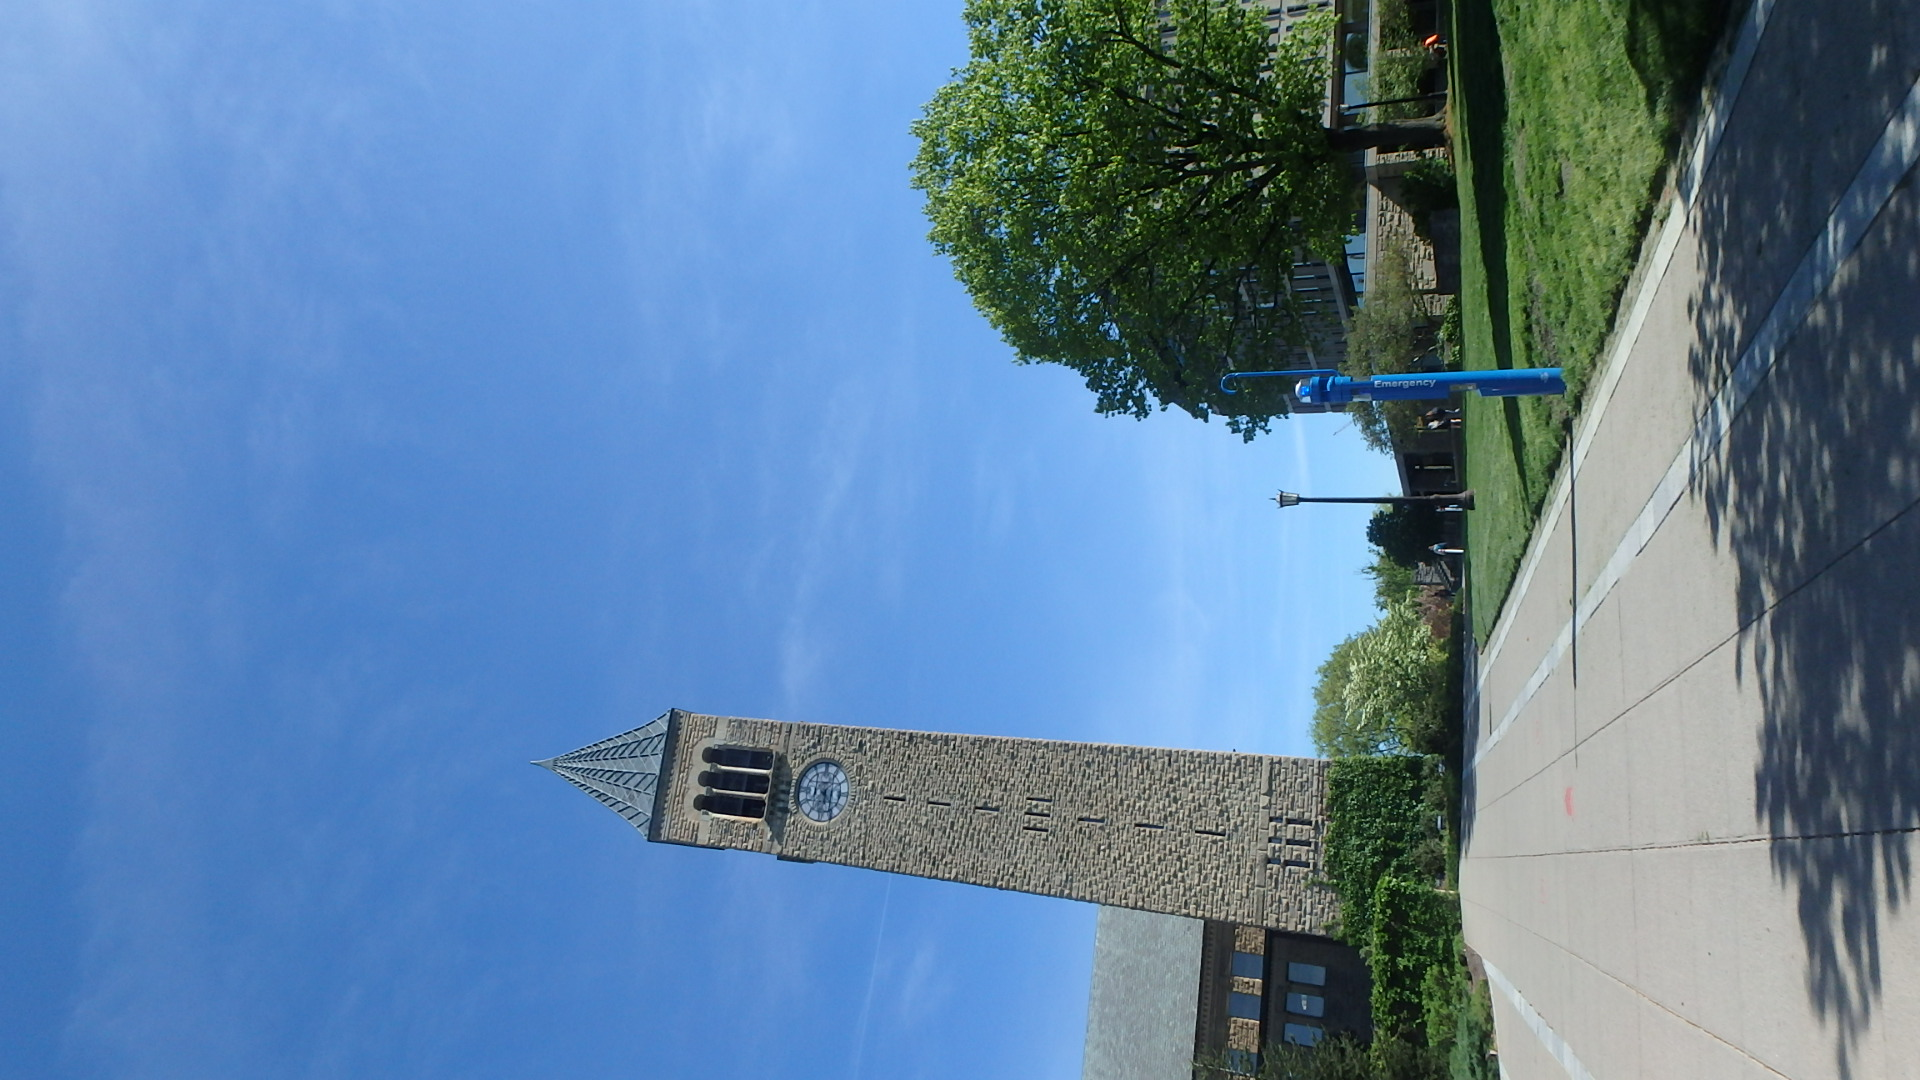
\includegraphics[scale=0.1,angle=-90]{chess1.JPG}
	\end{minipage}
	\begin{minipage}{0.5\textwidth}
	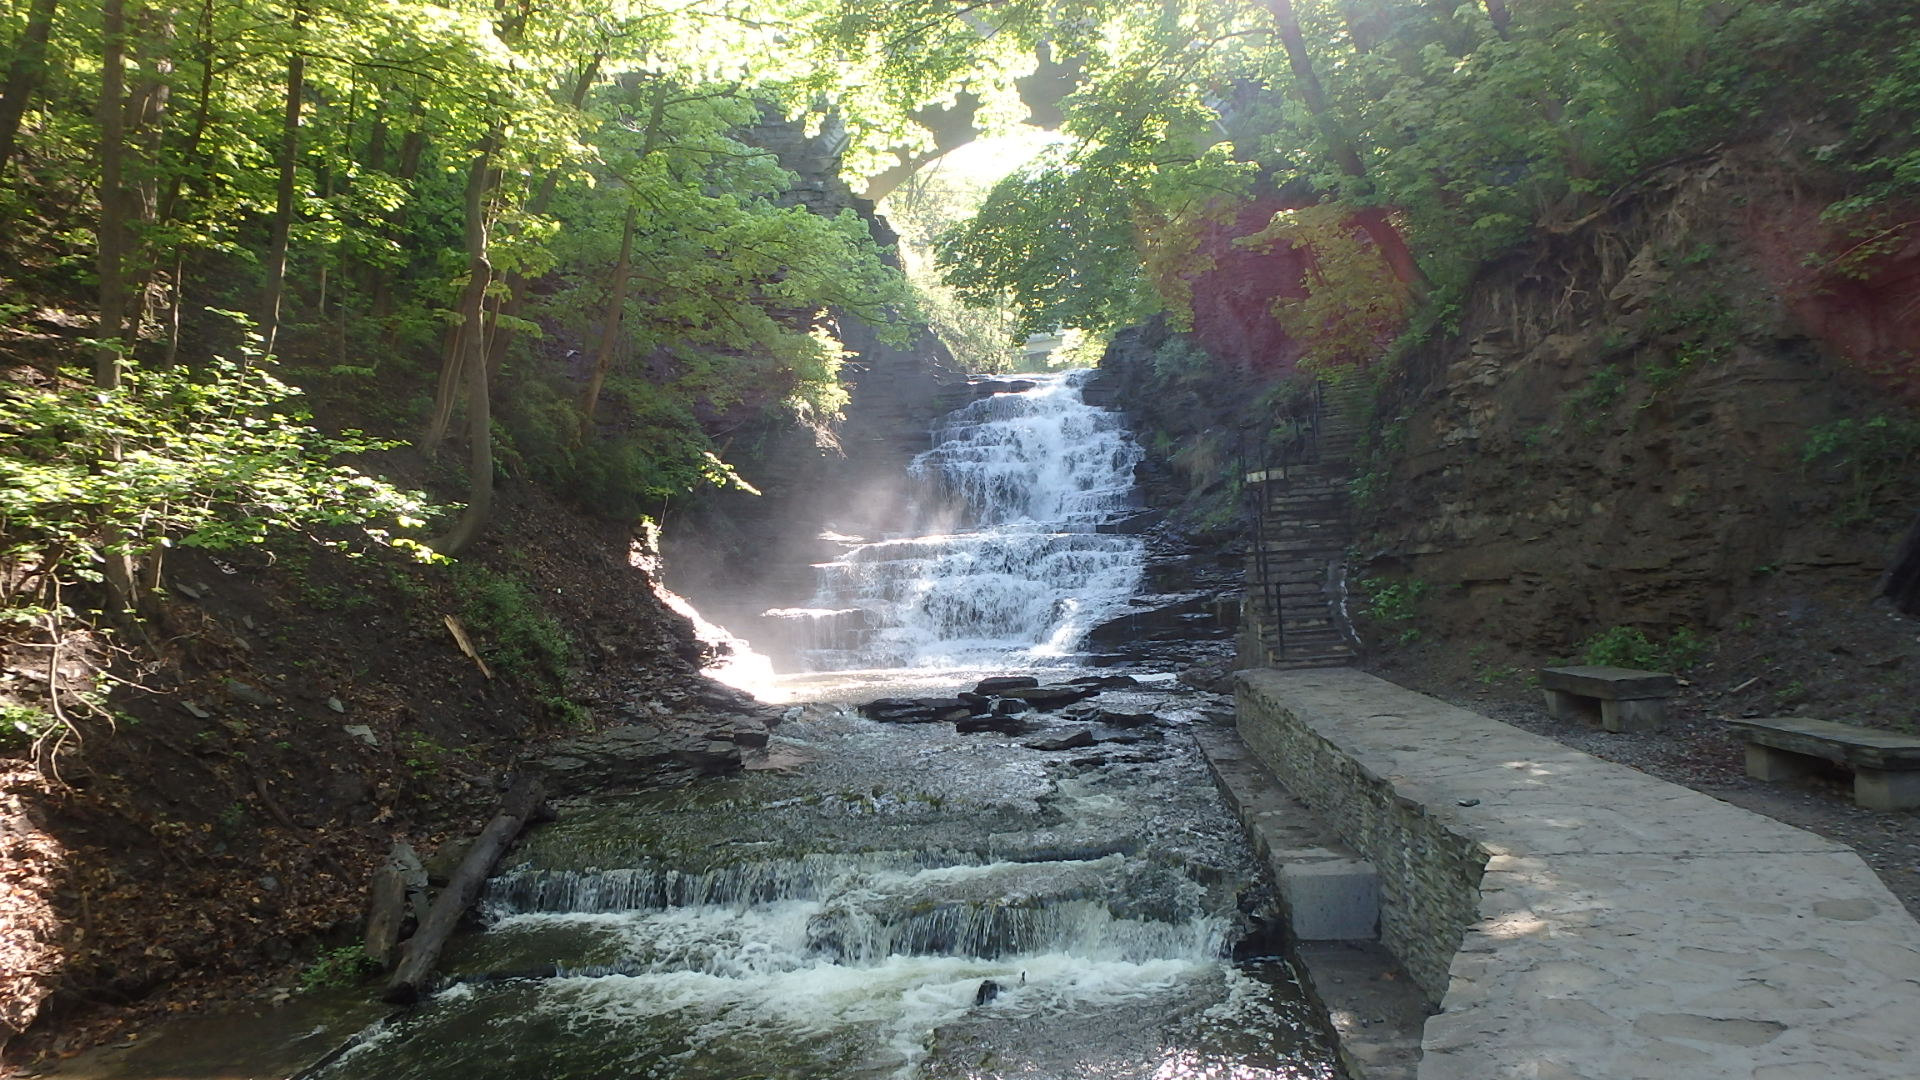
\includegraphics[scale=0.1]{chess2.JPG}
	\end{minipage}

\end{figure}

	\end{frame}
	
	\begin{frame}{Cornell High Energy Synchrotron Source (CHESS)}
	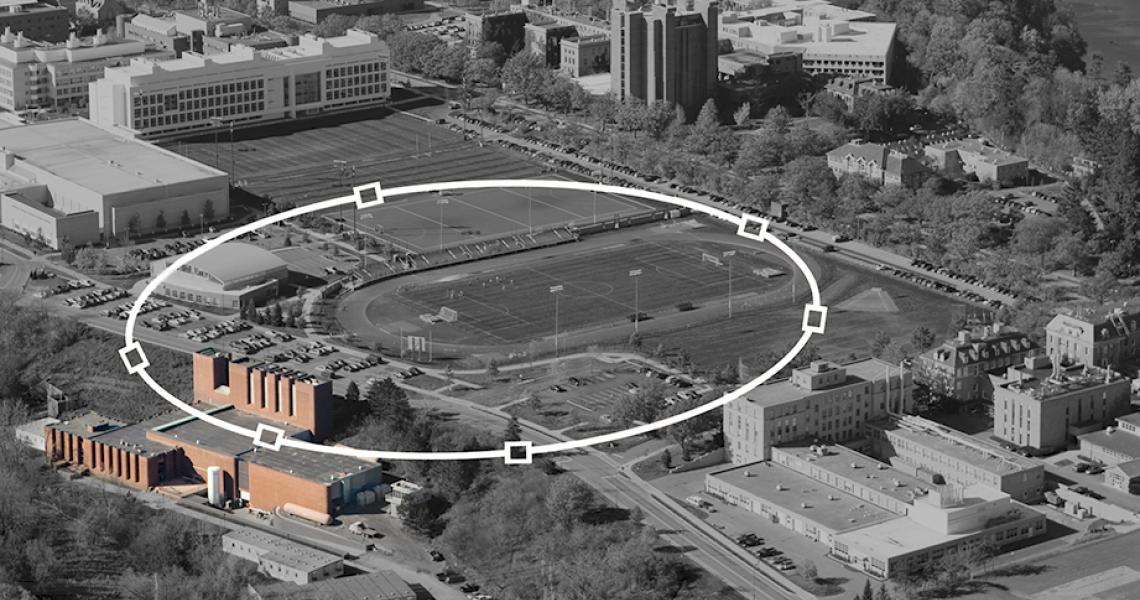
\includegraphics[width=\textwidth]{Ring.jpg}
	\end{frame}

	\begin{frame}{Synchrotron Tunnel}



\begin{figure}
	\begin{minipage}{0.47\textwidth}
		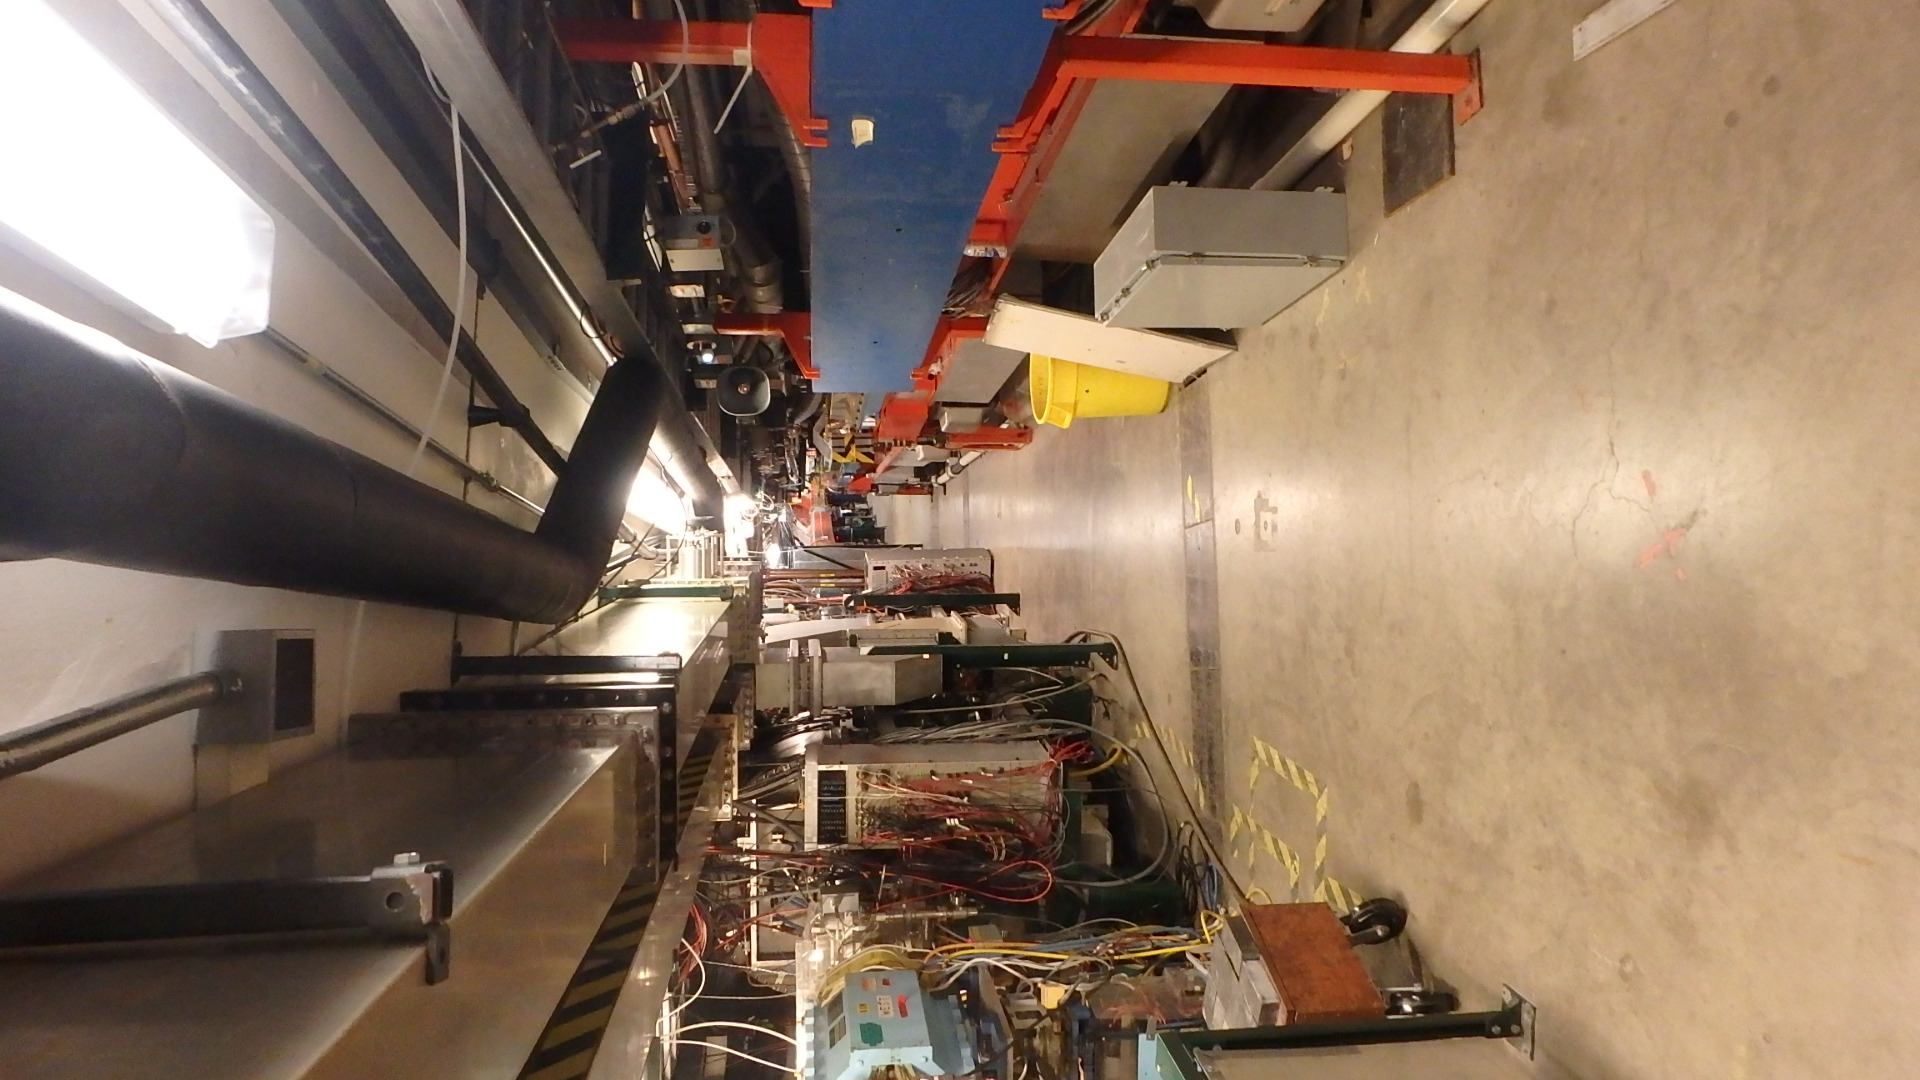
\includegraphics[scale=0.1,angle=-90]{chess4.JPG}
	\end{minipage}
	\begin{minipage}{0.5\textwidth}
		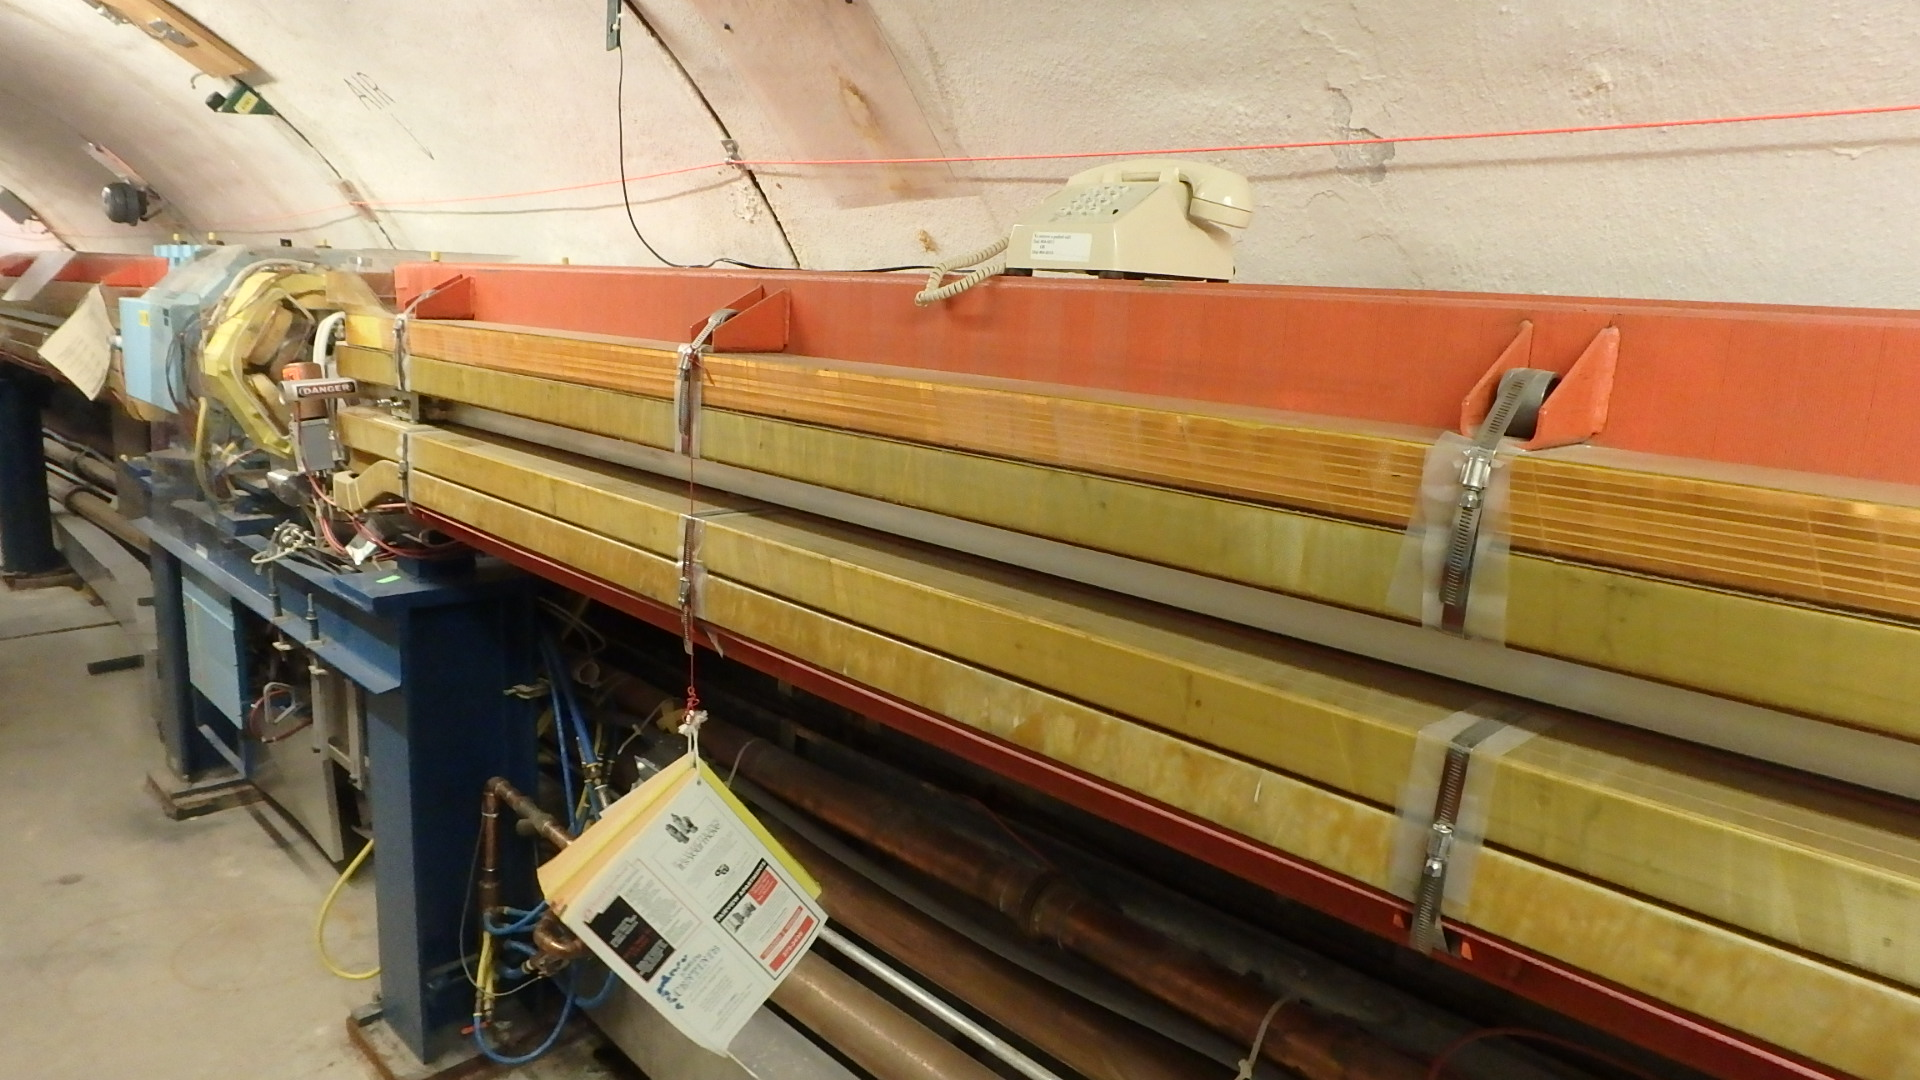
\includegraphics[scale=0.09]{chess5.JPG}
	\end{minipage}
	
\end{figure}

\end{frame}

\begin{frame}{D-Line}
\begin{figure}
	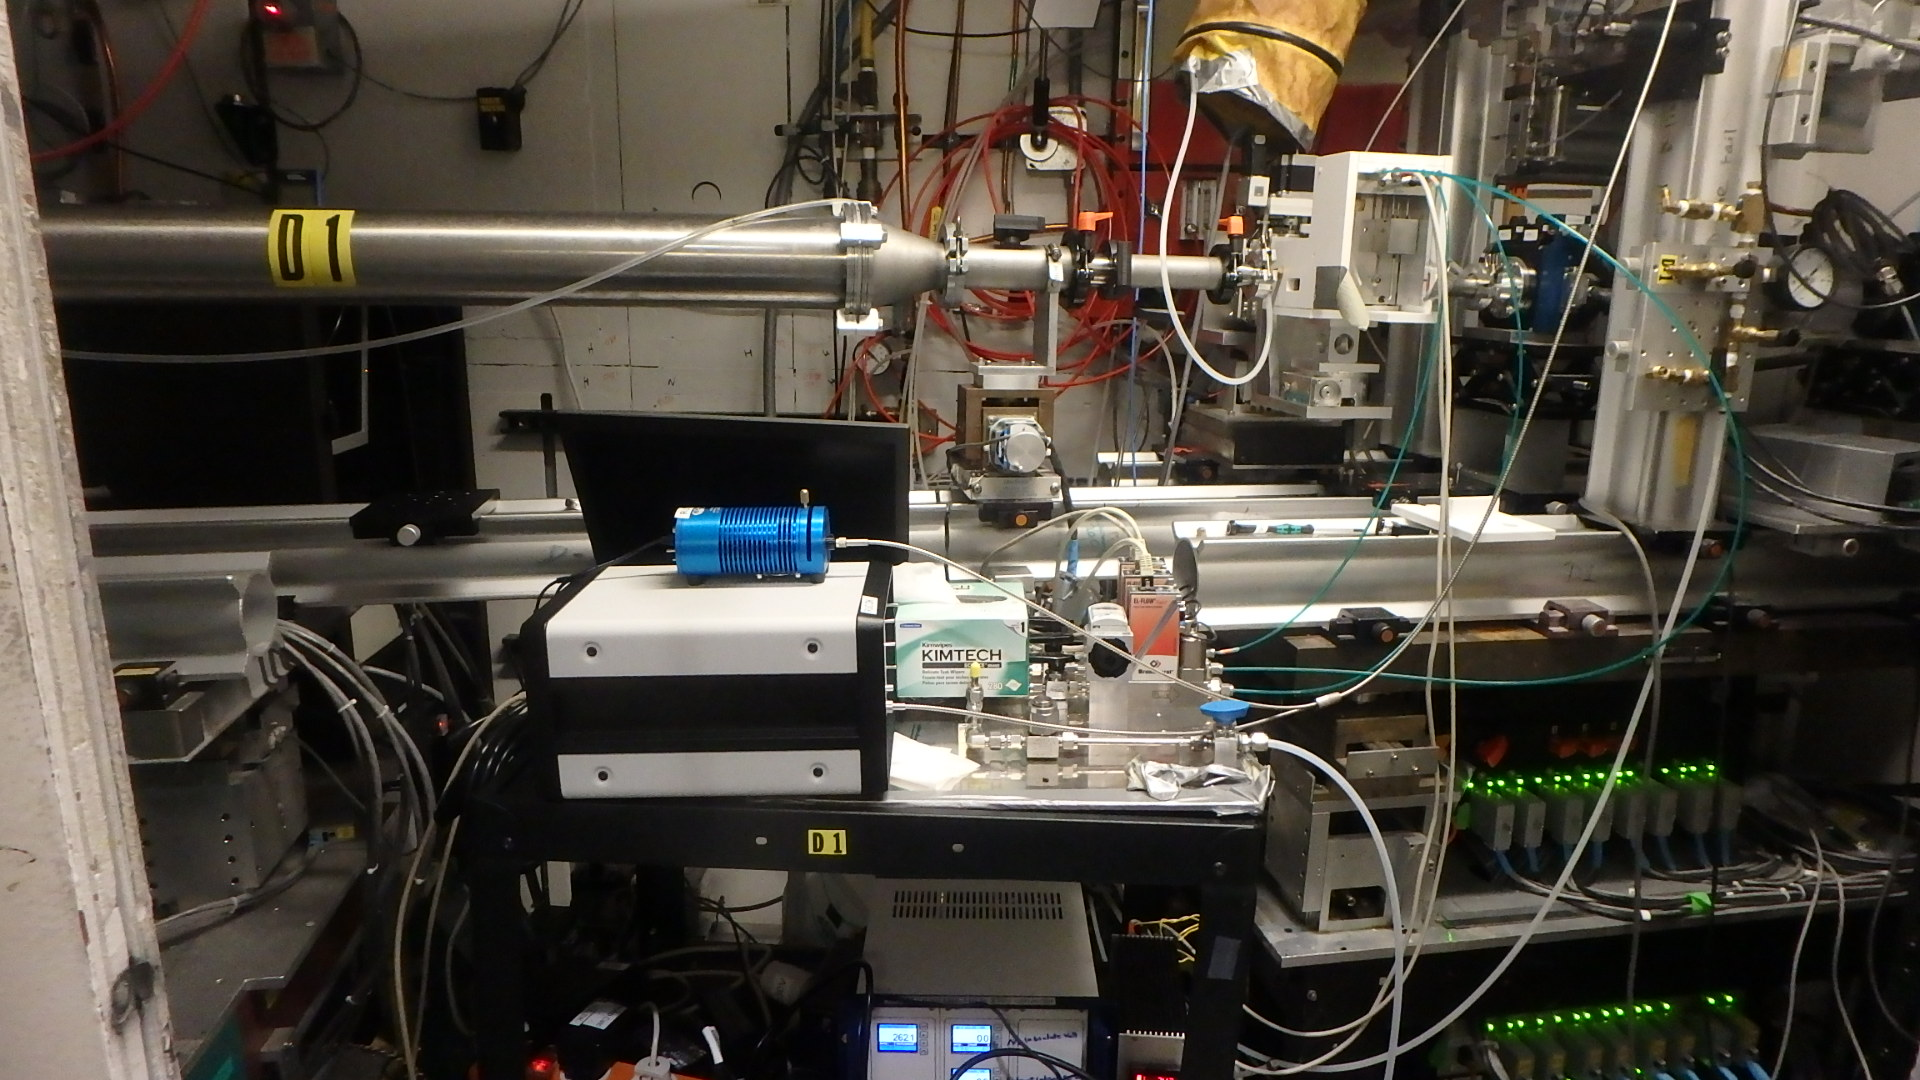
\includegraphics[scale=0.15]{chess3.JPG}
\end{figure}
\end{frame}

%	\begin{frame}{Thin Film Thickness}
%	
%	\begin{minipage}{0.47\textwidth}
%	    \begin{itemize}
%	    \item Experimental techniques: Atomic Force Microscopy, Ellipsometry and x-ray reflectometry
%	    \item Spectroscopic Reflectometry
%	    \begin{itemize}
%	    \item In-situ
%	    \item Harsh environment
%	    \item Small enough for test chamber and testing stage
%	    \end{itemize}
%	    \item Complement GISAXS measurements 
%	    \end{itemize}
%	\end{minipage}
%	\begin{minipage}{0.5\textwidth}
%	    \begin{figure}
%	    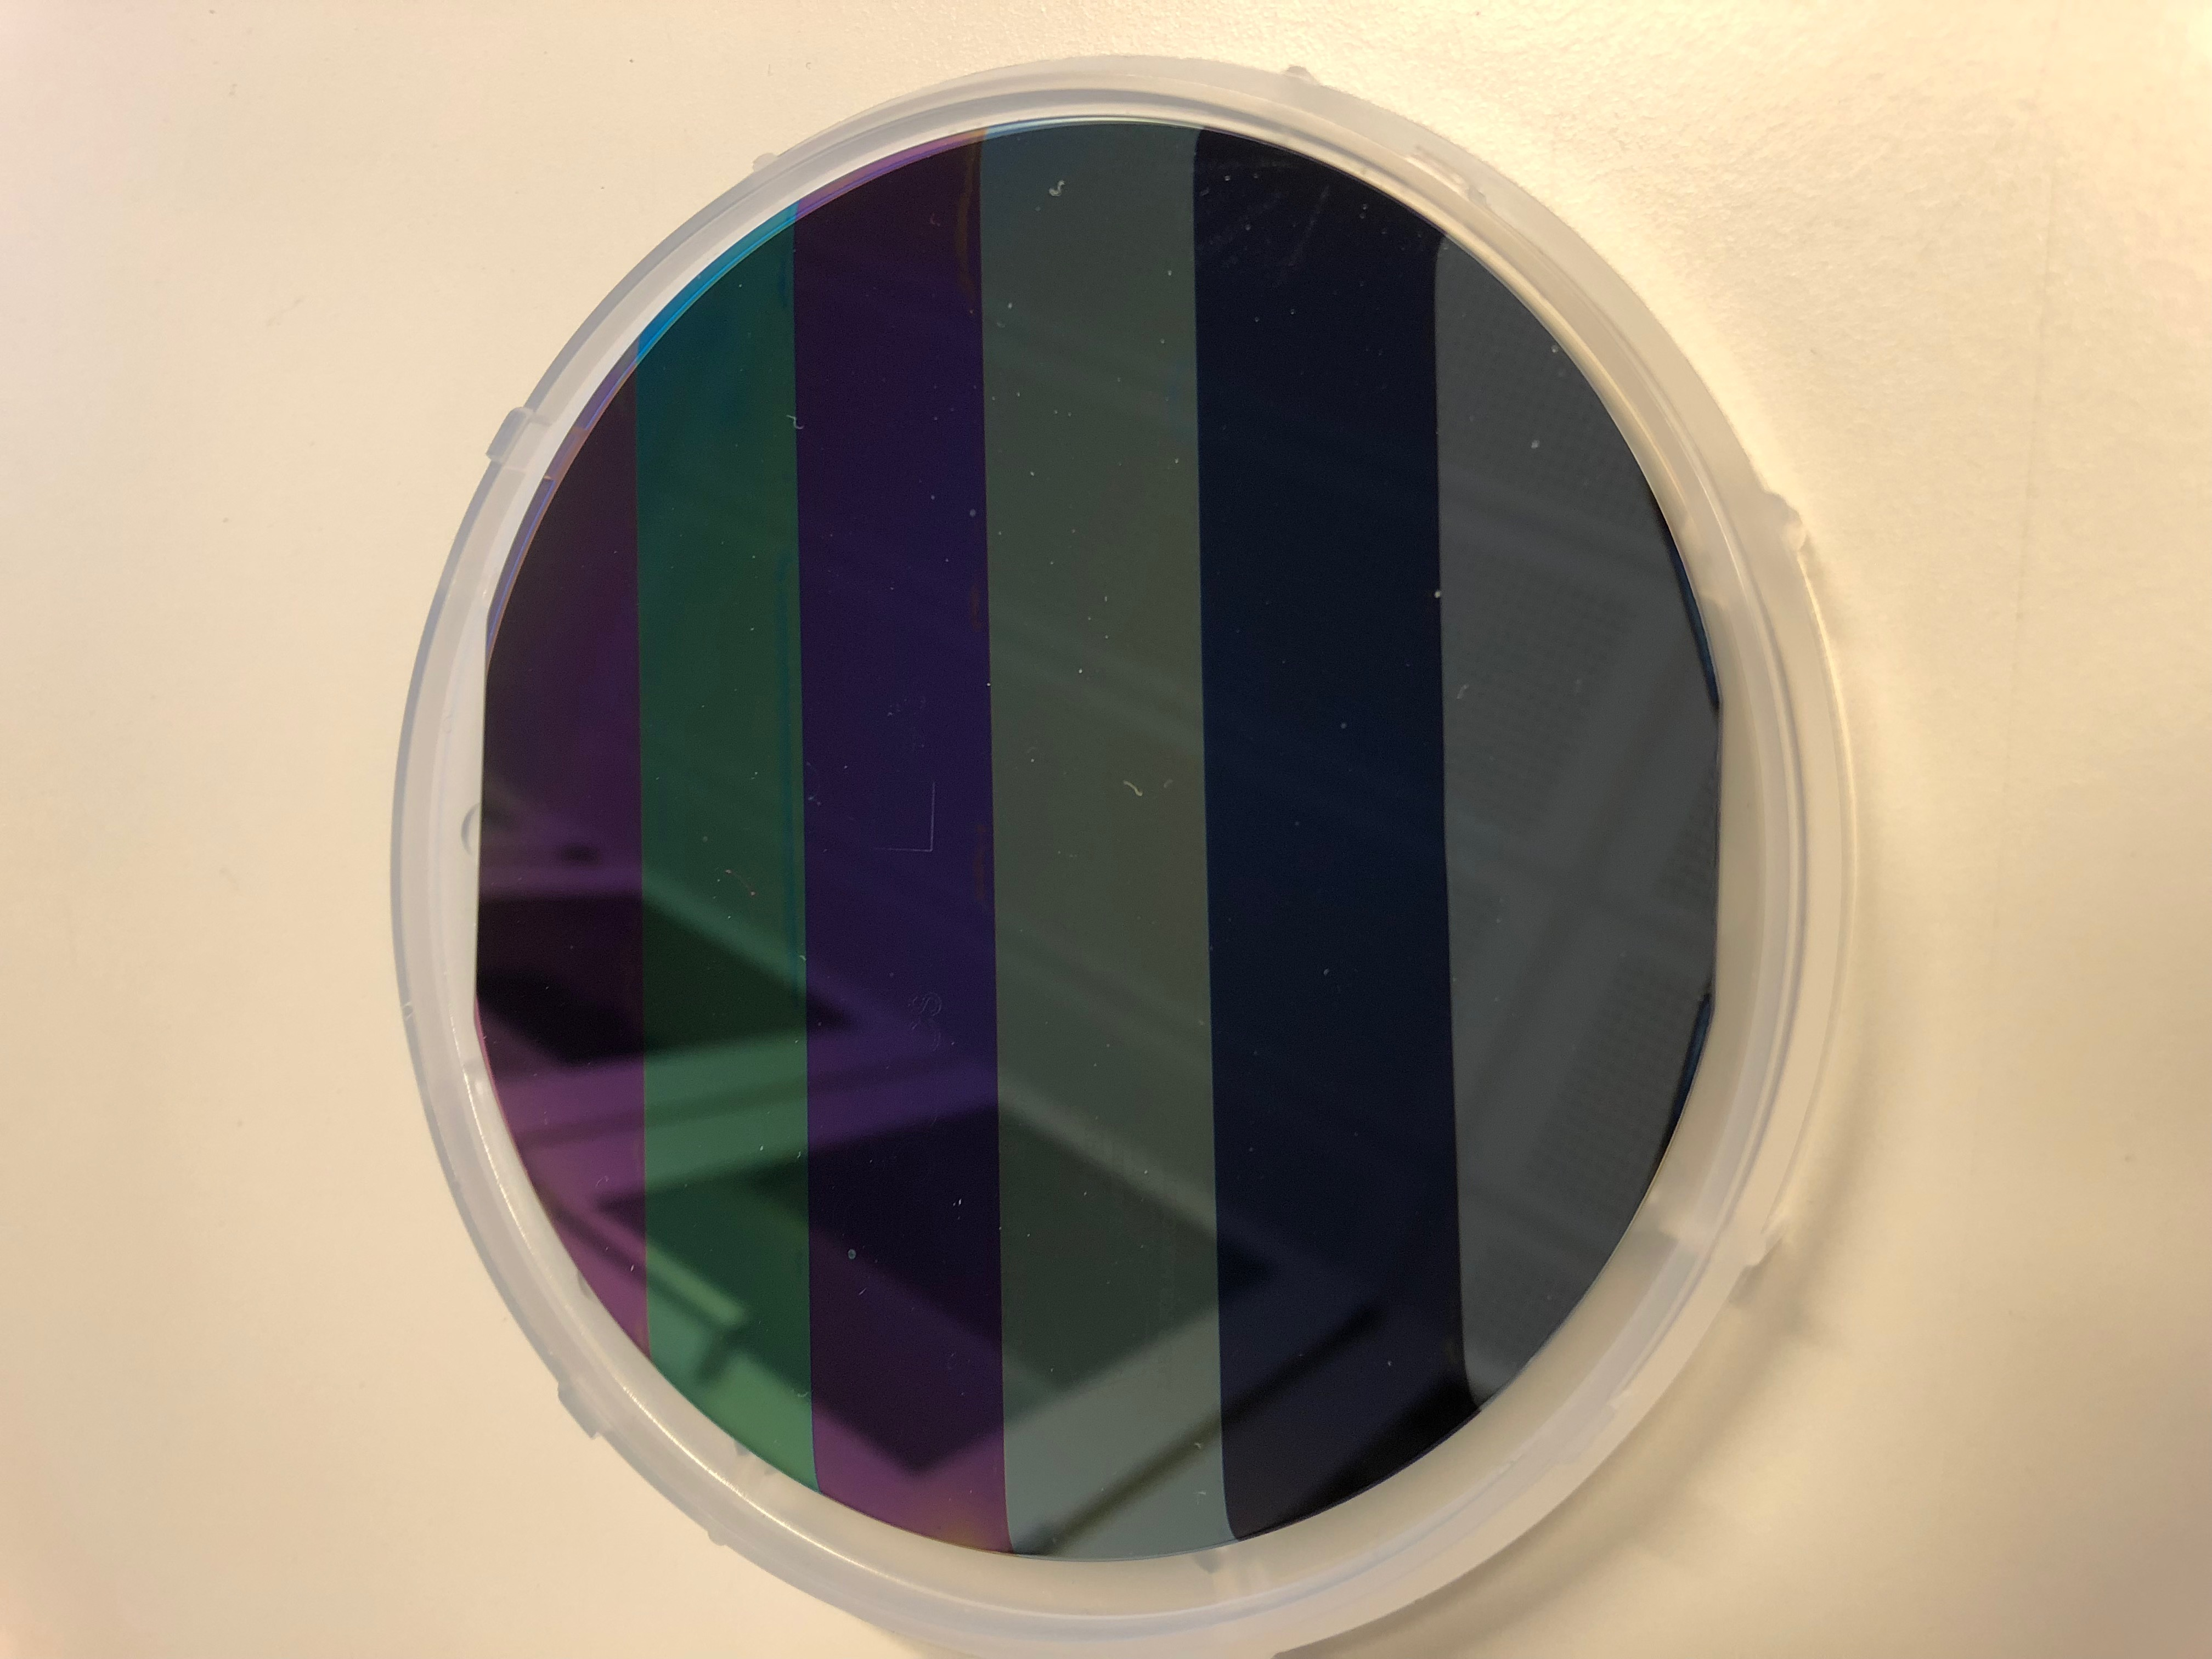
\includegraphics[scale=0.025,angle=-90]{stepwafer.JPG}
%	    \end{figure}
%	\end{minipage}
%	\end{frame}
	
	
		\section{Experimental Setup}
		
		\begin{frame}{Components}
		NanoCalc XR, Halogen Light Source, Test Chamber and Single Point Stage
		
		\begin{minipage}{0.47\textwidth}
		\begin{figure}
		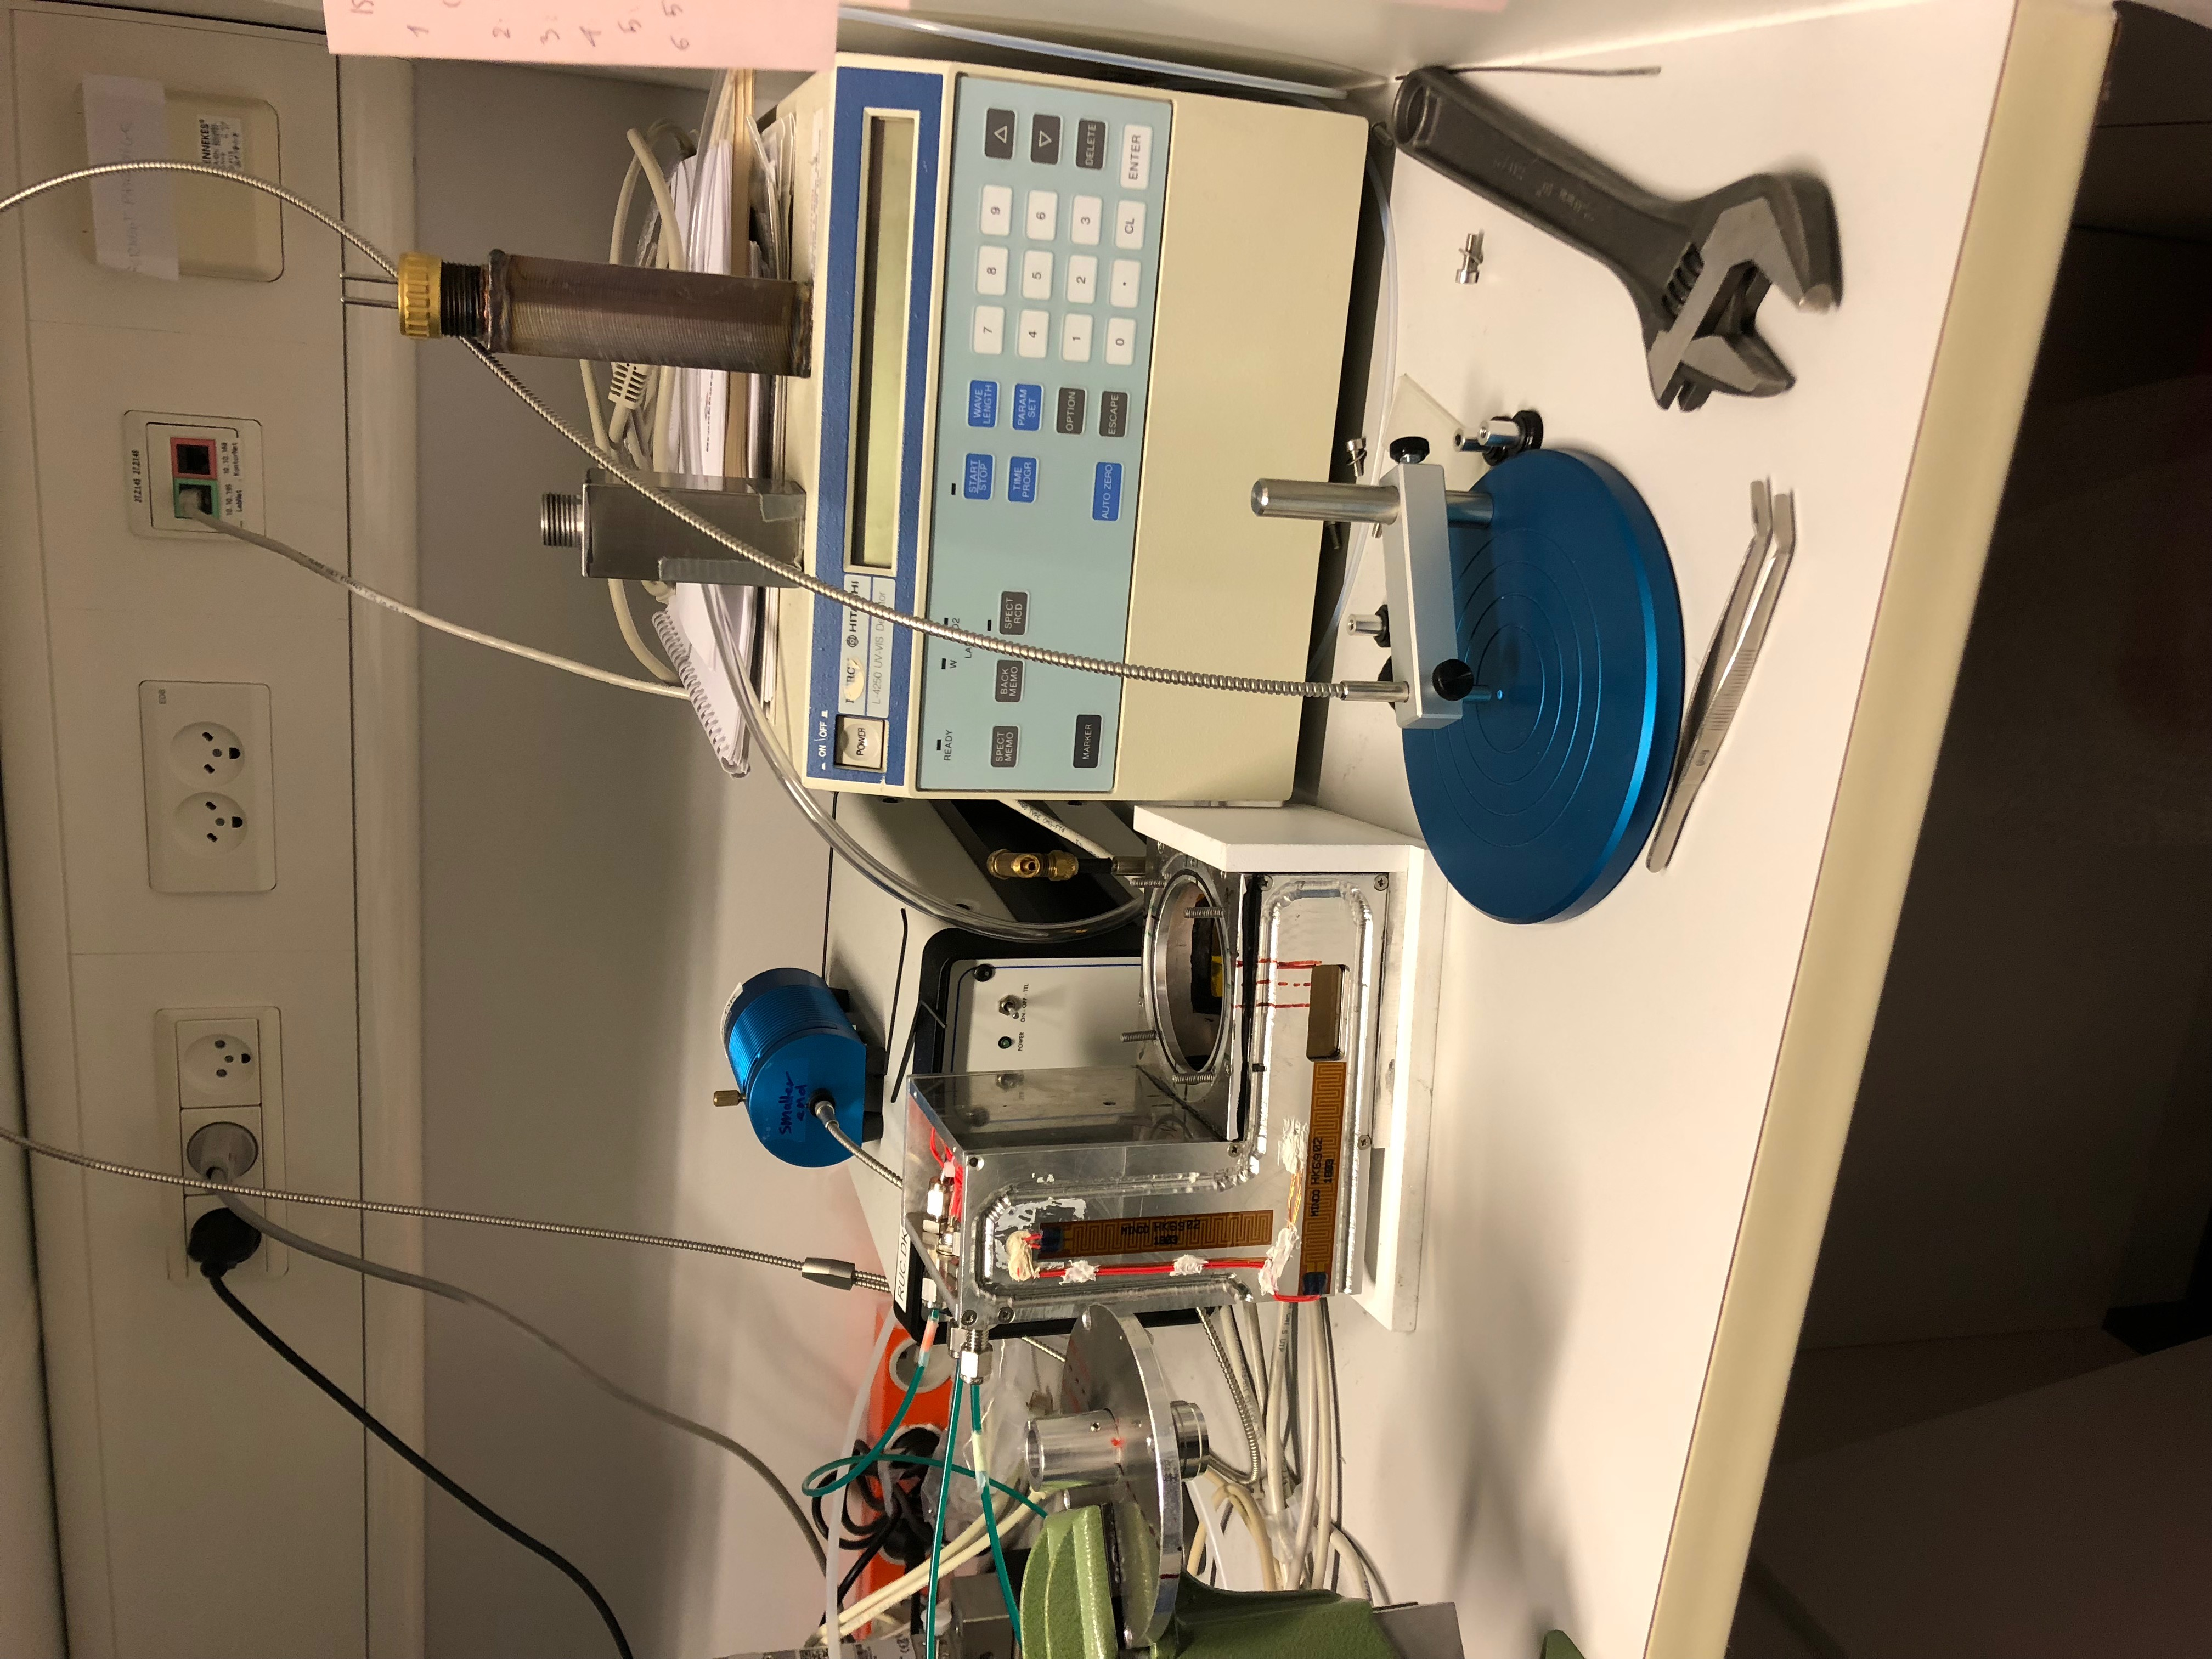
\includegraphics[scale=0.04,angle=-90]{setup1.JPG}
		\end{figure}
		\end{minipage}
		\begin{minipage}{0.5\textwidth}
		\begin{figure}
		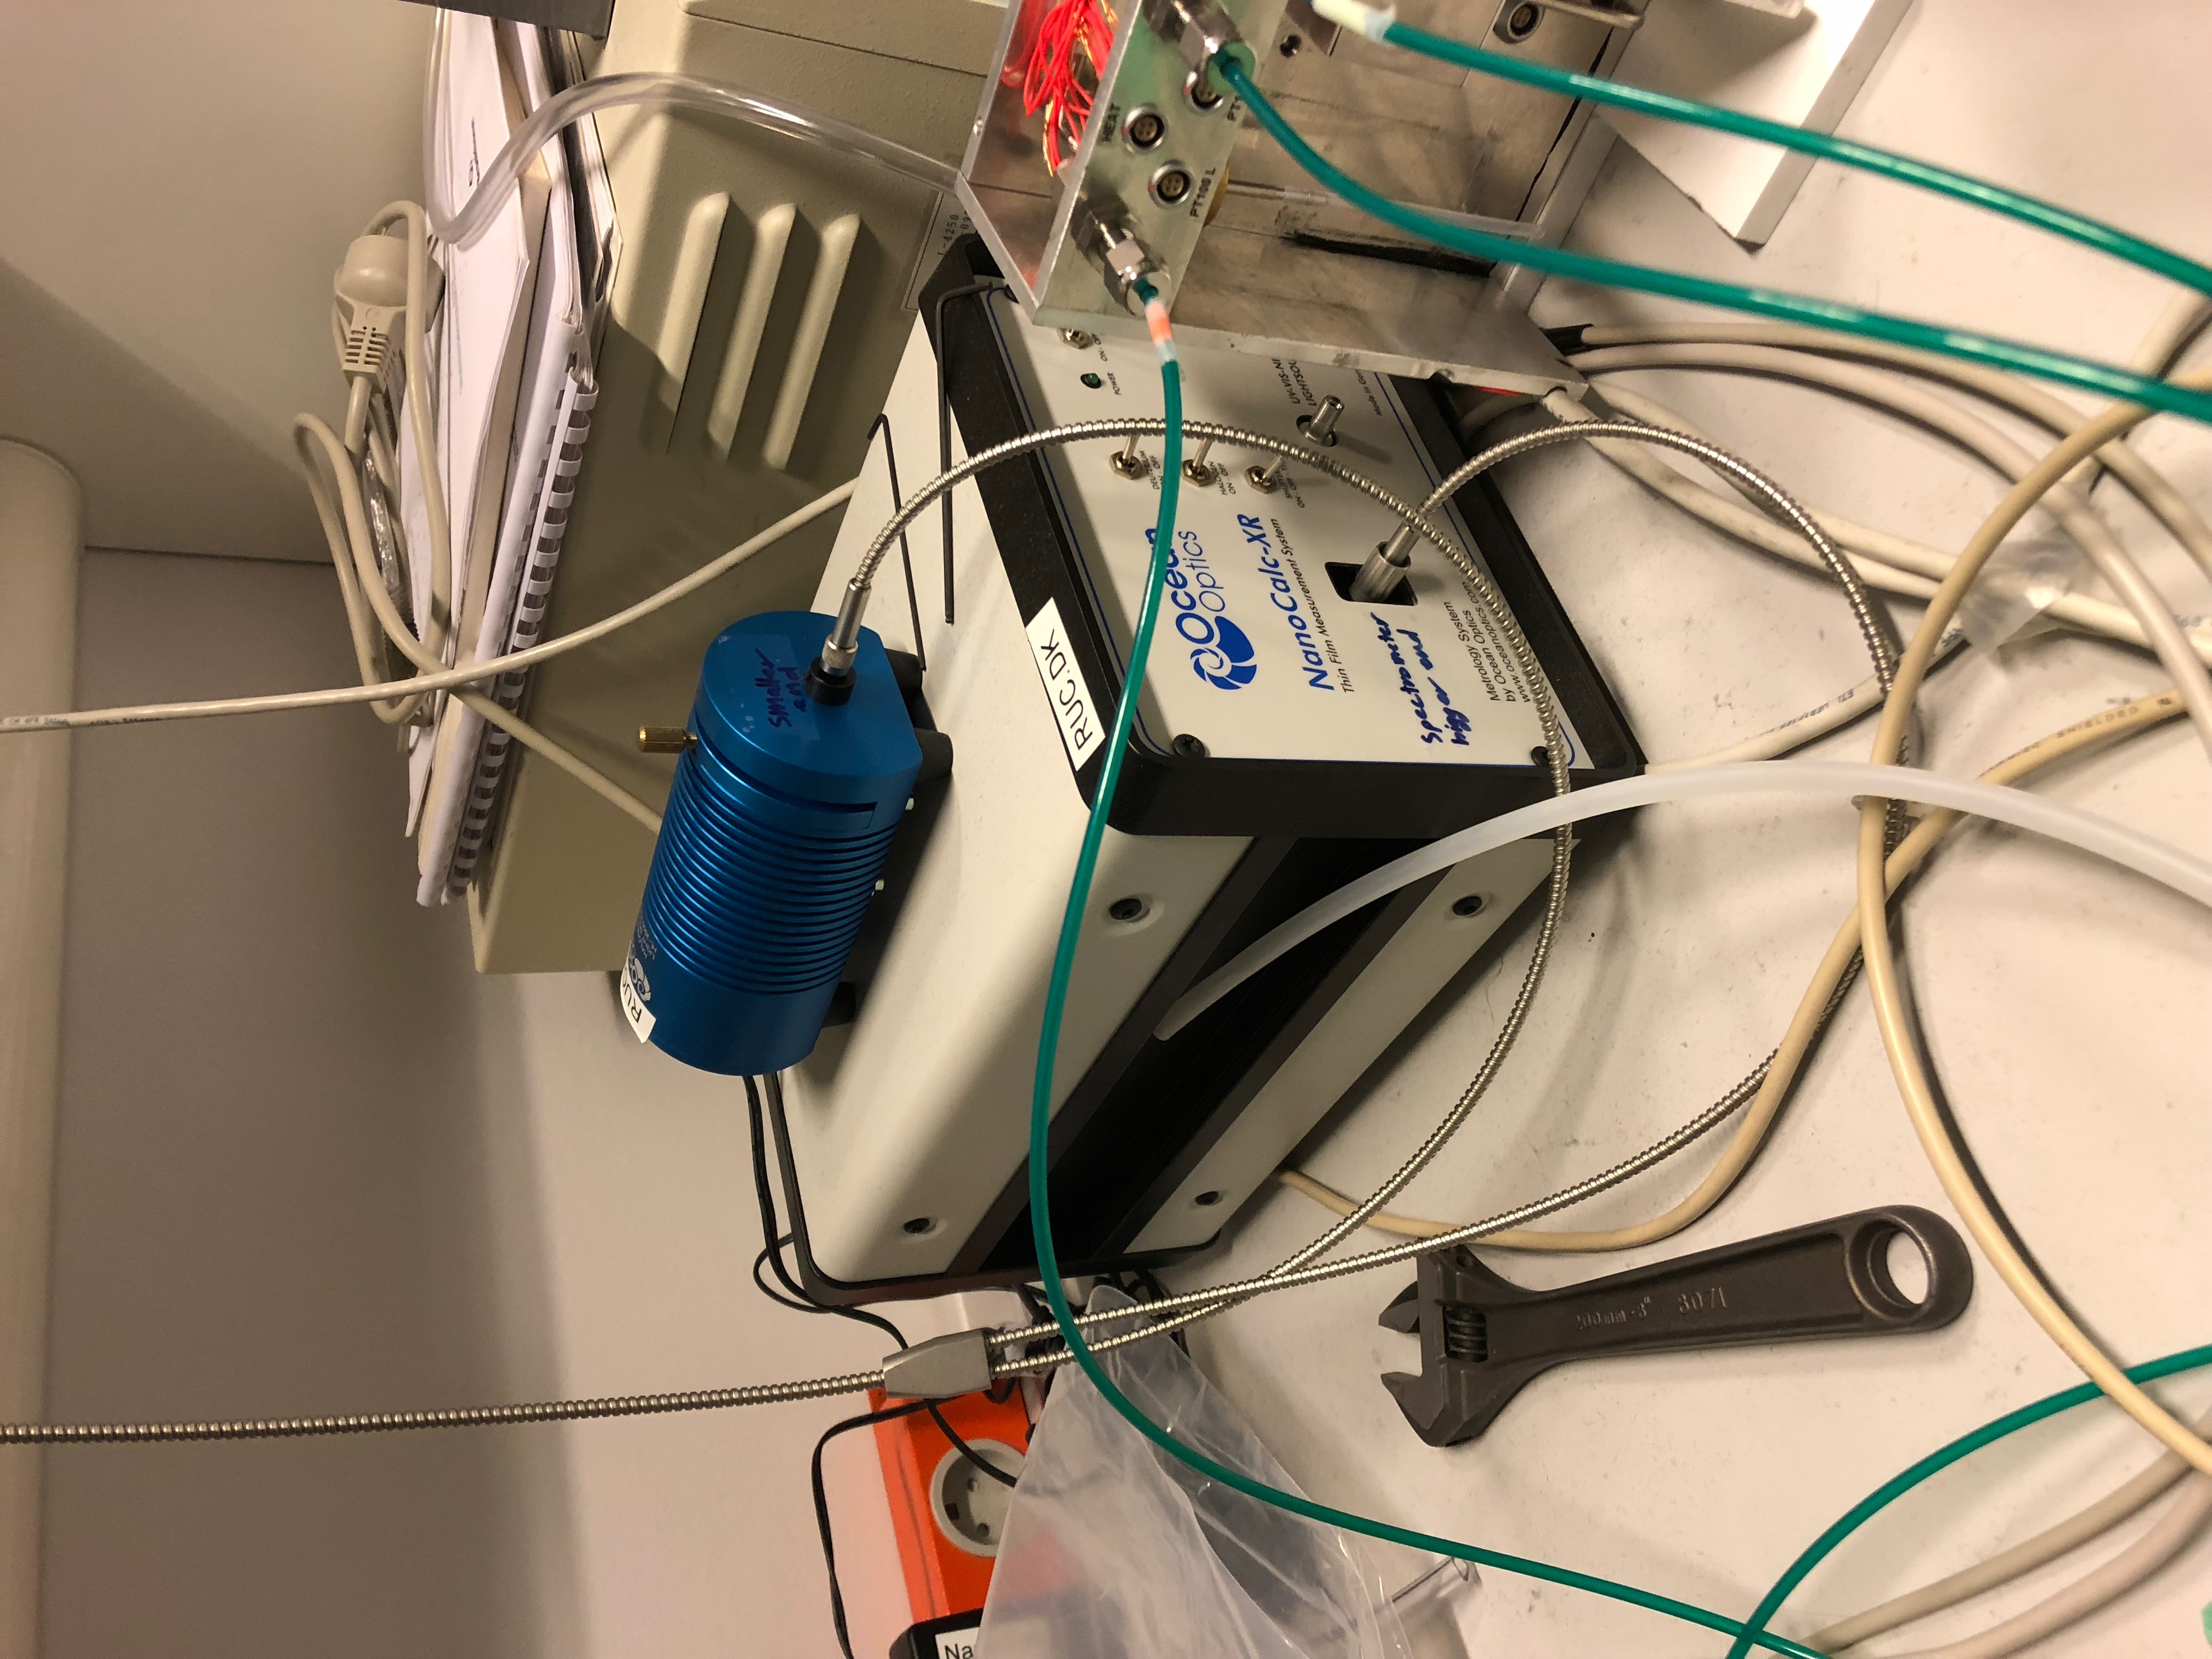
\includegraphics[scale=0.04,angle=-90]{setup2.JPG}
		\end{figure}
		\end{minipage}
	
		\end{frame}
		
		\begin{frame}{Components Cont.}
		\begin{minipage}{0.47\textwidth}
		\begin{figure}
		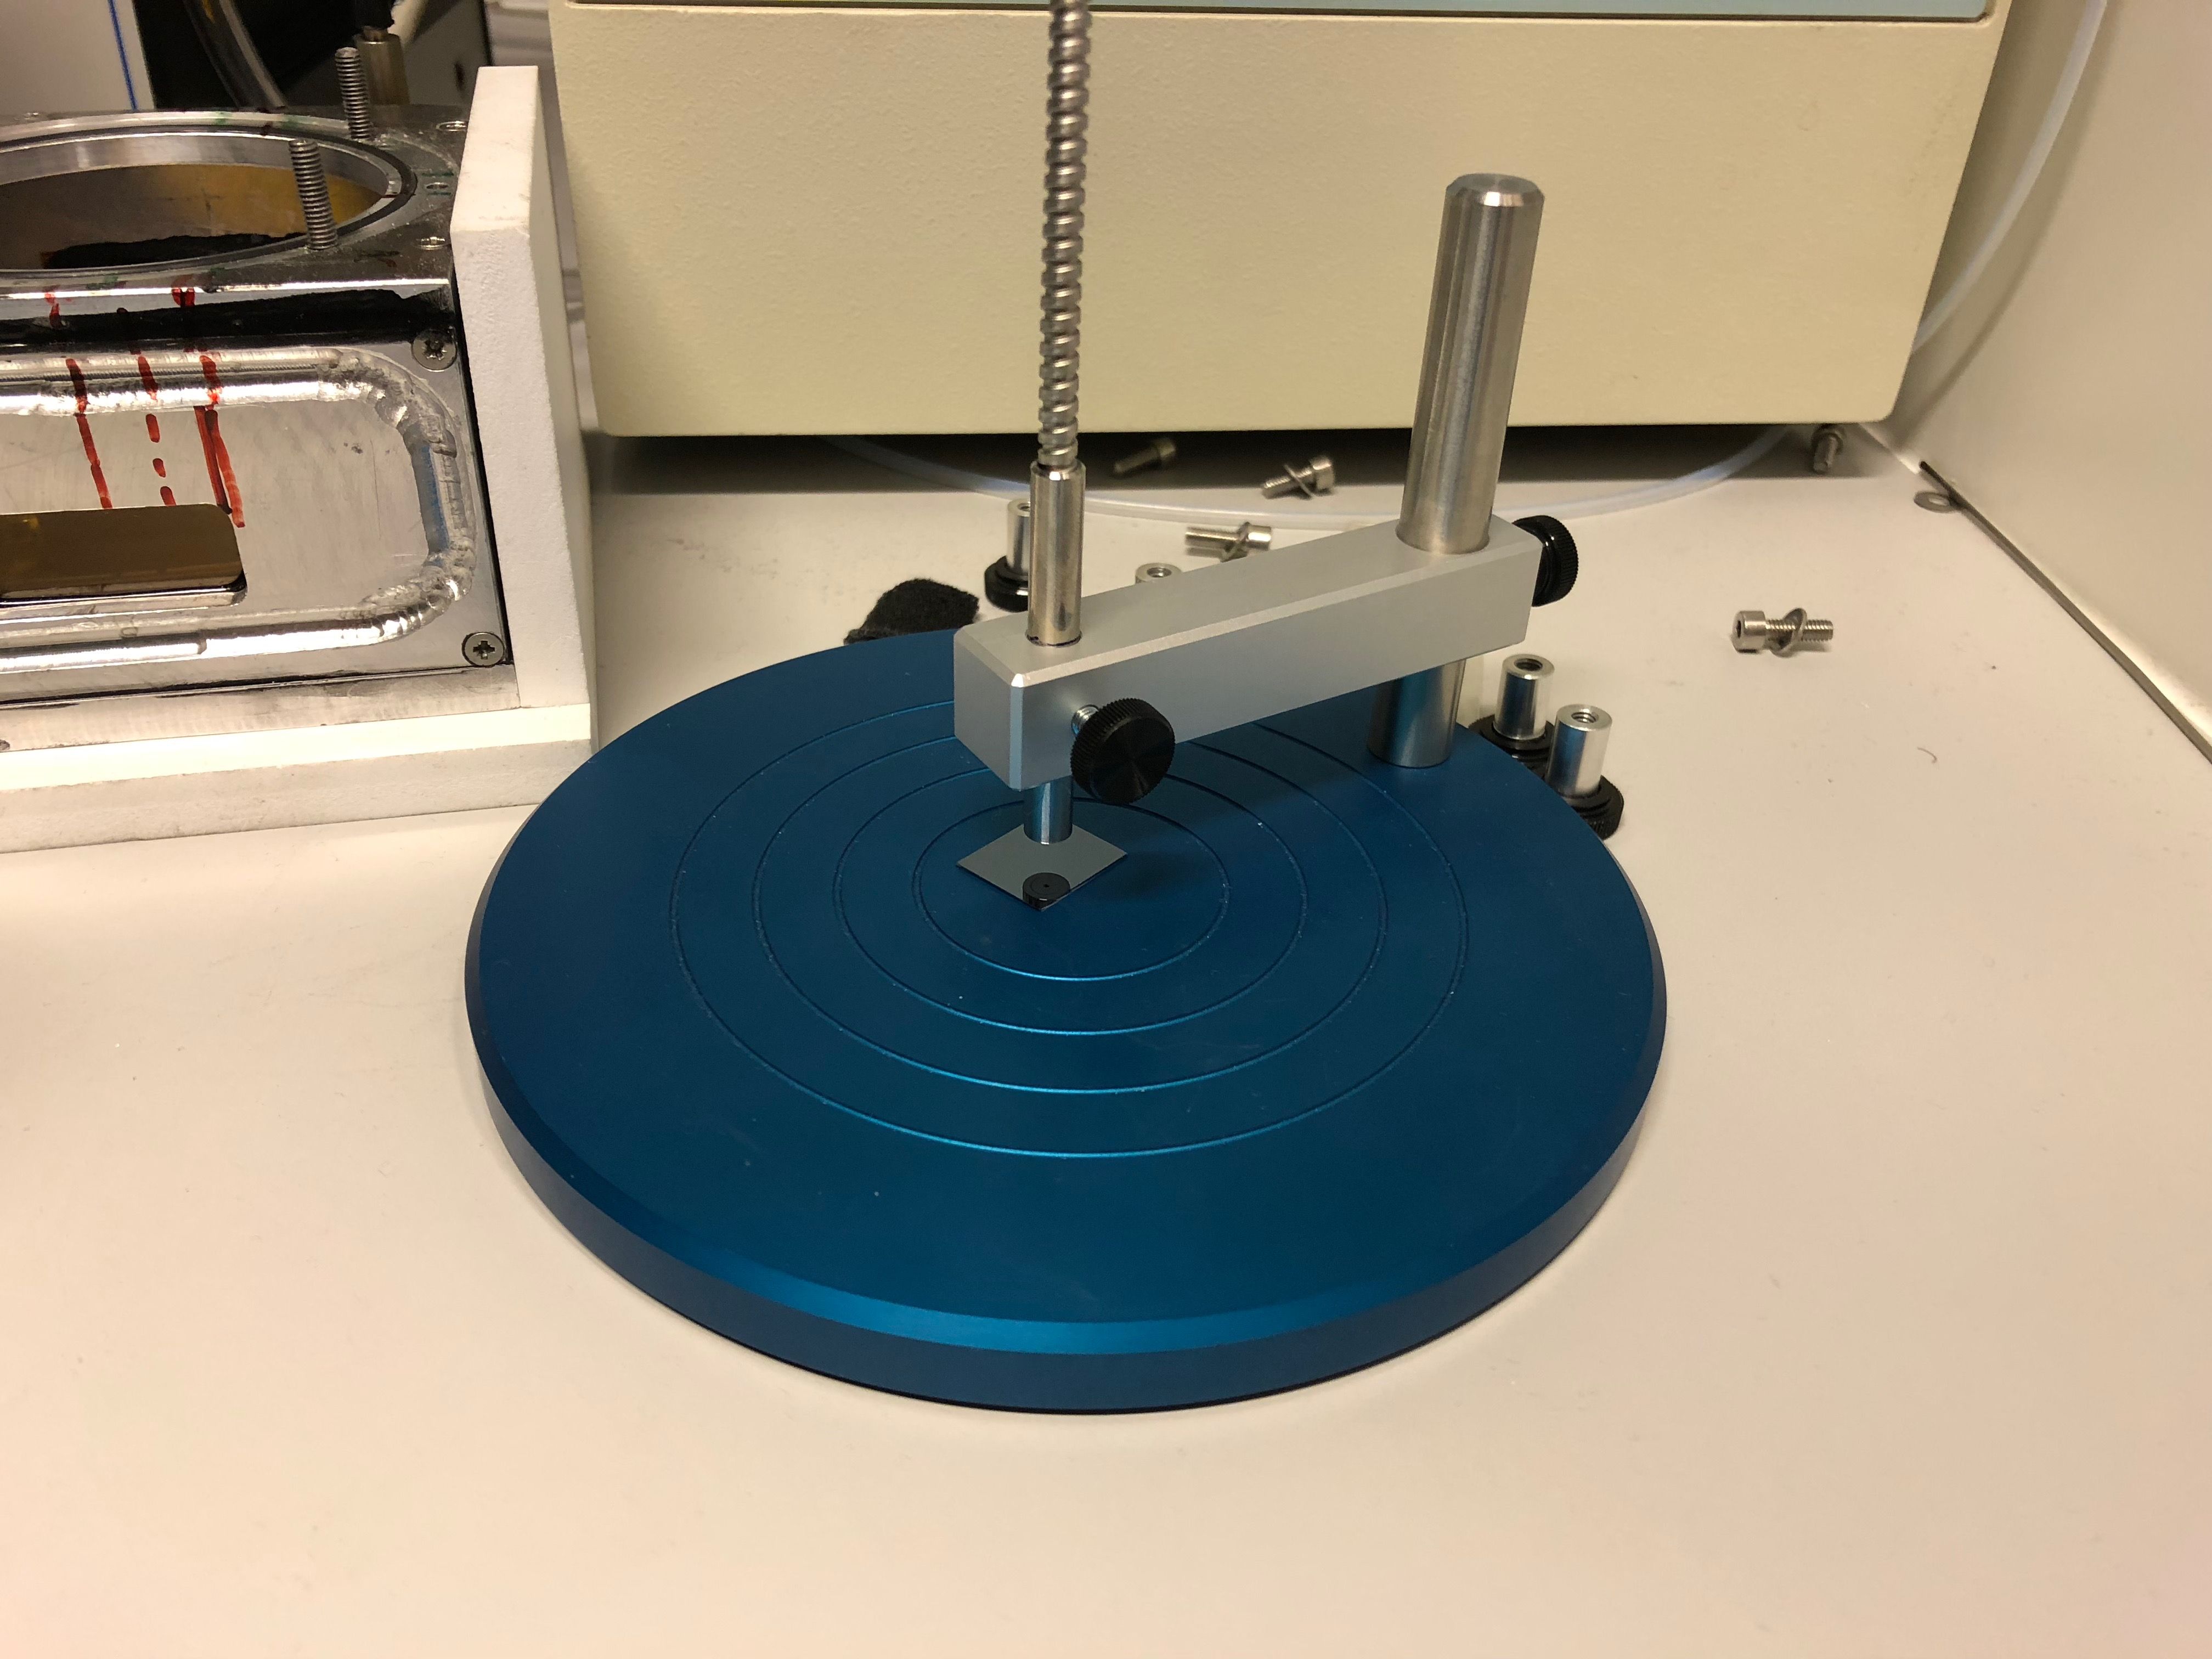
\includegraphics[scale=0.04]{setup3.JPG}
		\end{figure}
		\end{minipage}
		\begin{minipage}{0.5\textwidth}
		\begin{figure}
		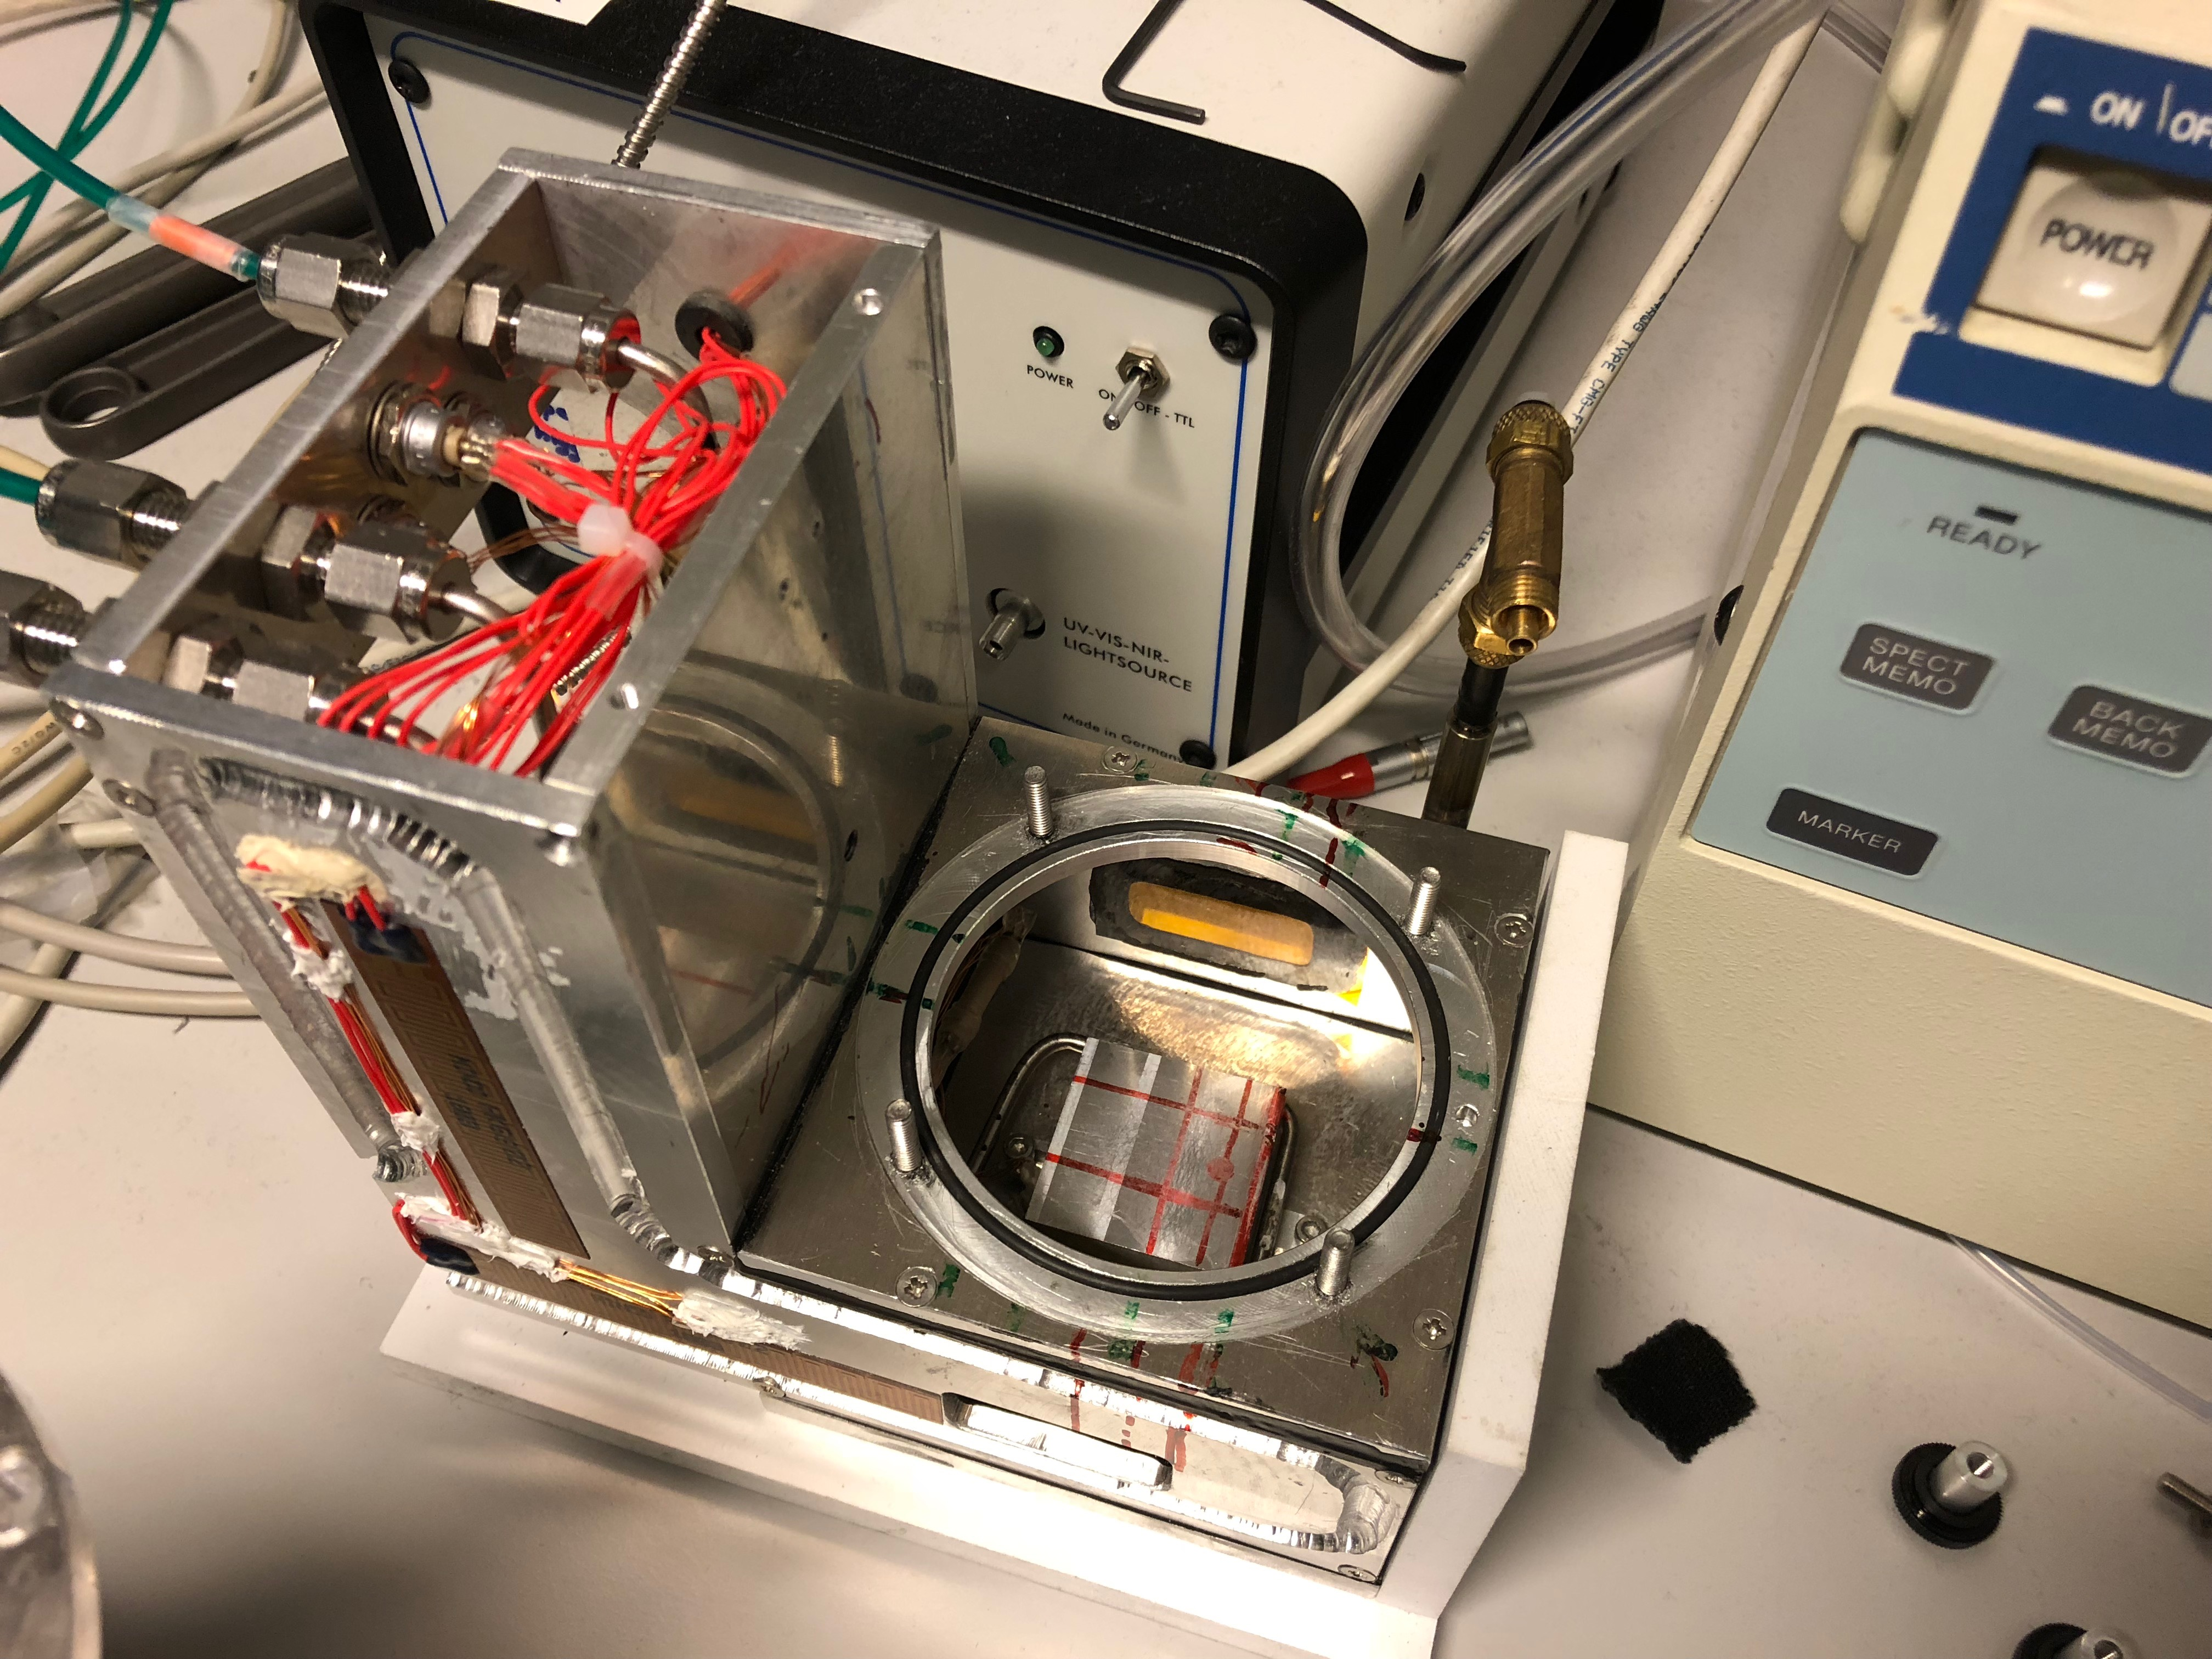
\includegraphics[scale=0.04]{setup4.JPG}
		\end{figure}
		\end{minipage}
		\end{frame}
	
	\section{Problem Formulation}
	\begin{frame}{Problem Formulation}
	What can White Light Spectroscopic Reflectometry infer with respect to SVA swelling experiments using the homopolymers: Polystyrene, Polyisoprene and Poly(methyl methacrylate)? 
	
	Can the same modelling of homopolymers be used with respect to Polystyrene-b-Polyisoprene?
	
	Model:
	\begin{itemize}
	\item Change in refractive index of the ambient 
	\item Change in refractive index of the thinfilm
	\item In-situ thickness measurements
	\end{itemize}  
	\end{frame}
	

	
	\section{Light}
	\begin{frame}{Electromagnetic Radiation}
	\begin{minipage}{0.47\textwidth}
			\begin{figure}
			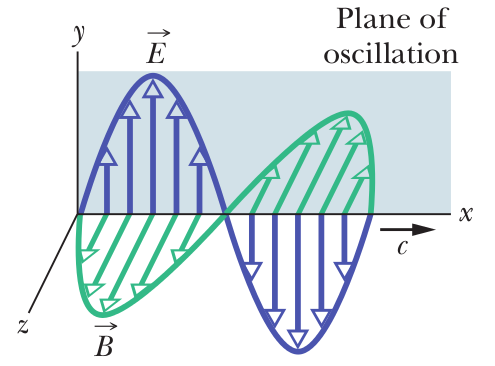
\includegraphics[scale=0.3]{EM.png}
			\end{figure}
			\end{minipage}
			\begin{minipage}{0.5\textwidth}
			\begin{figure}
			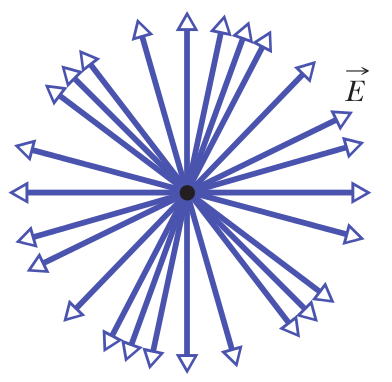
\includegraphics[scale=0.3]{unpol.png}
			\end{figure}
			\end{minipage}
	\end{frame}
	
	\begin{frame}{Light Spectrum and Spectrometer}
				\begin{minipage}{0.47\textwidth}
				\begin{figure}
				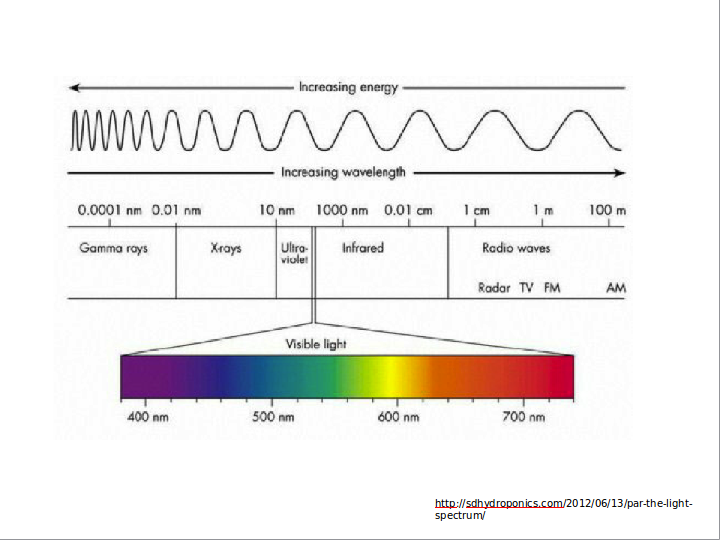
\includegraphics[scale=0.25]{light.png}
				\end{figure}
				\end{minipage}
				\begin{minipage}{0.5\textwidth}
				\begin{figure}
				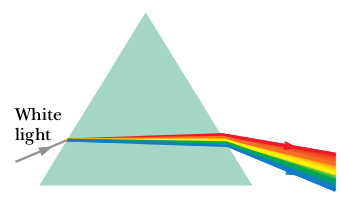
\includegraphics[scale=0.25]{prism.png}
				\end{figure}
				\begin{figure}
				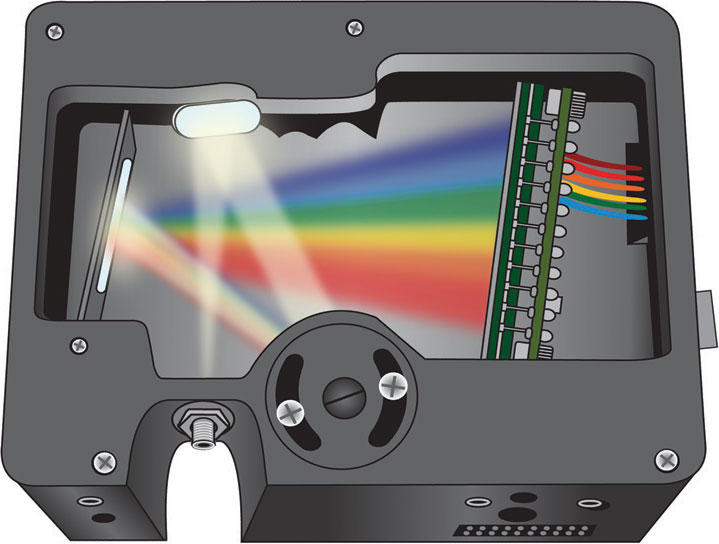
\includegraphics[scale=0.15]{spectrometer.jpg}
				\end{figure}
				\end{minipage}
	
	\end{frame}
	
	\begin{frame}{Thin Film Phenomena}
				\begin{minipage}{0.47\textwidth}
				\begin{figure}
				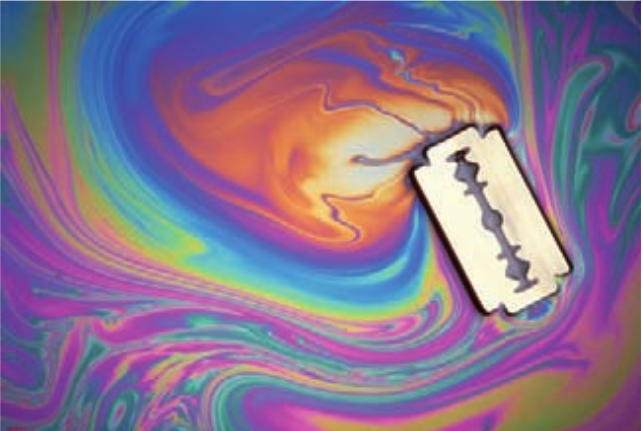
\includegraphics[scale=0.25]{soap.png}
				\end{figure}
				\end{minipage}
				\begin{minipage}{0.5\textwidth}
				\begin{figure}
				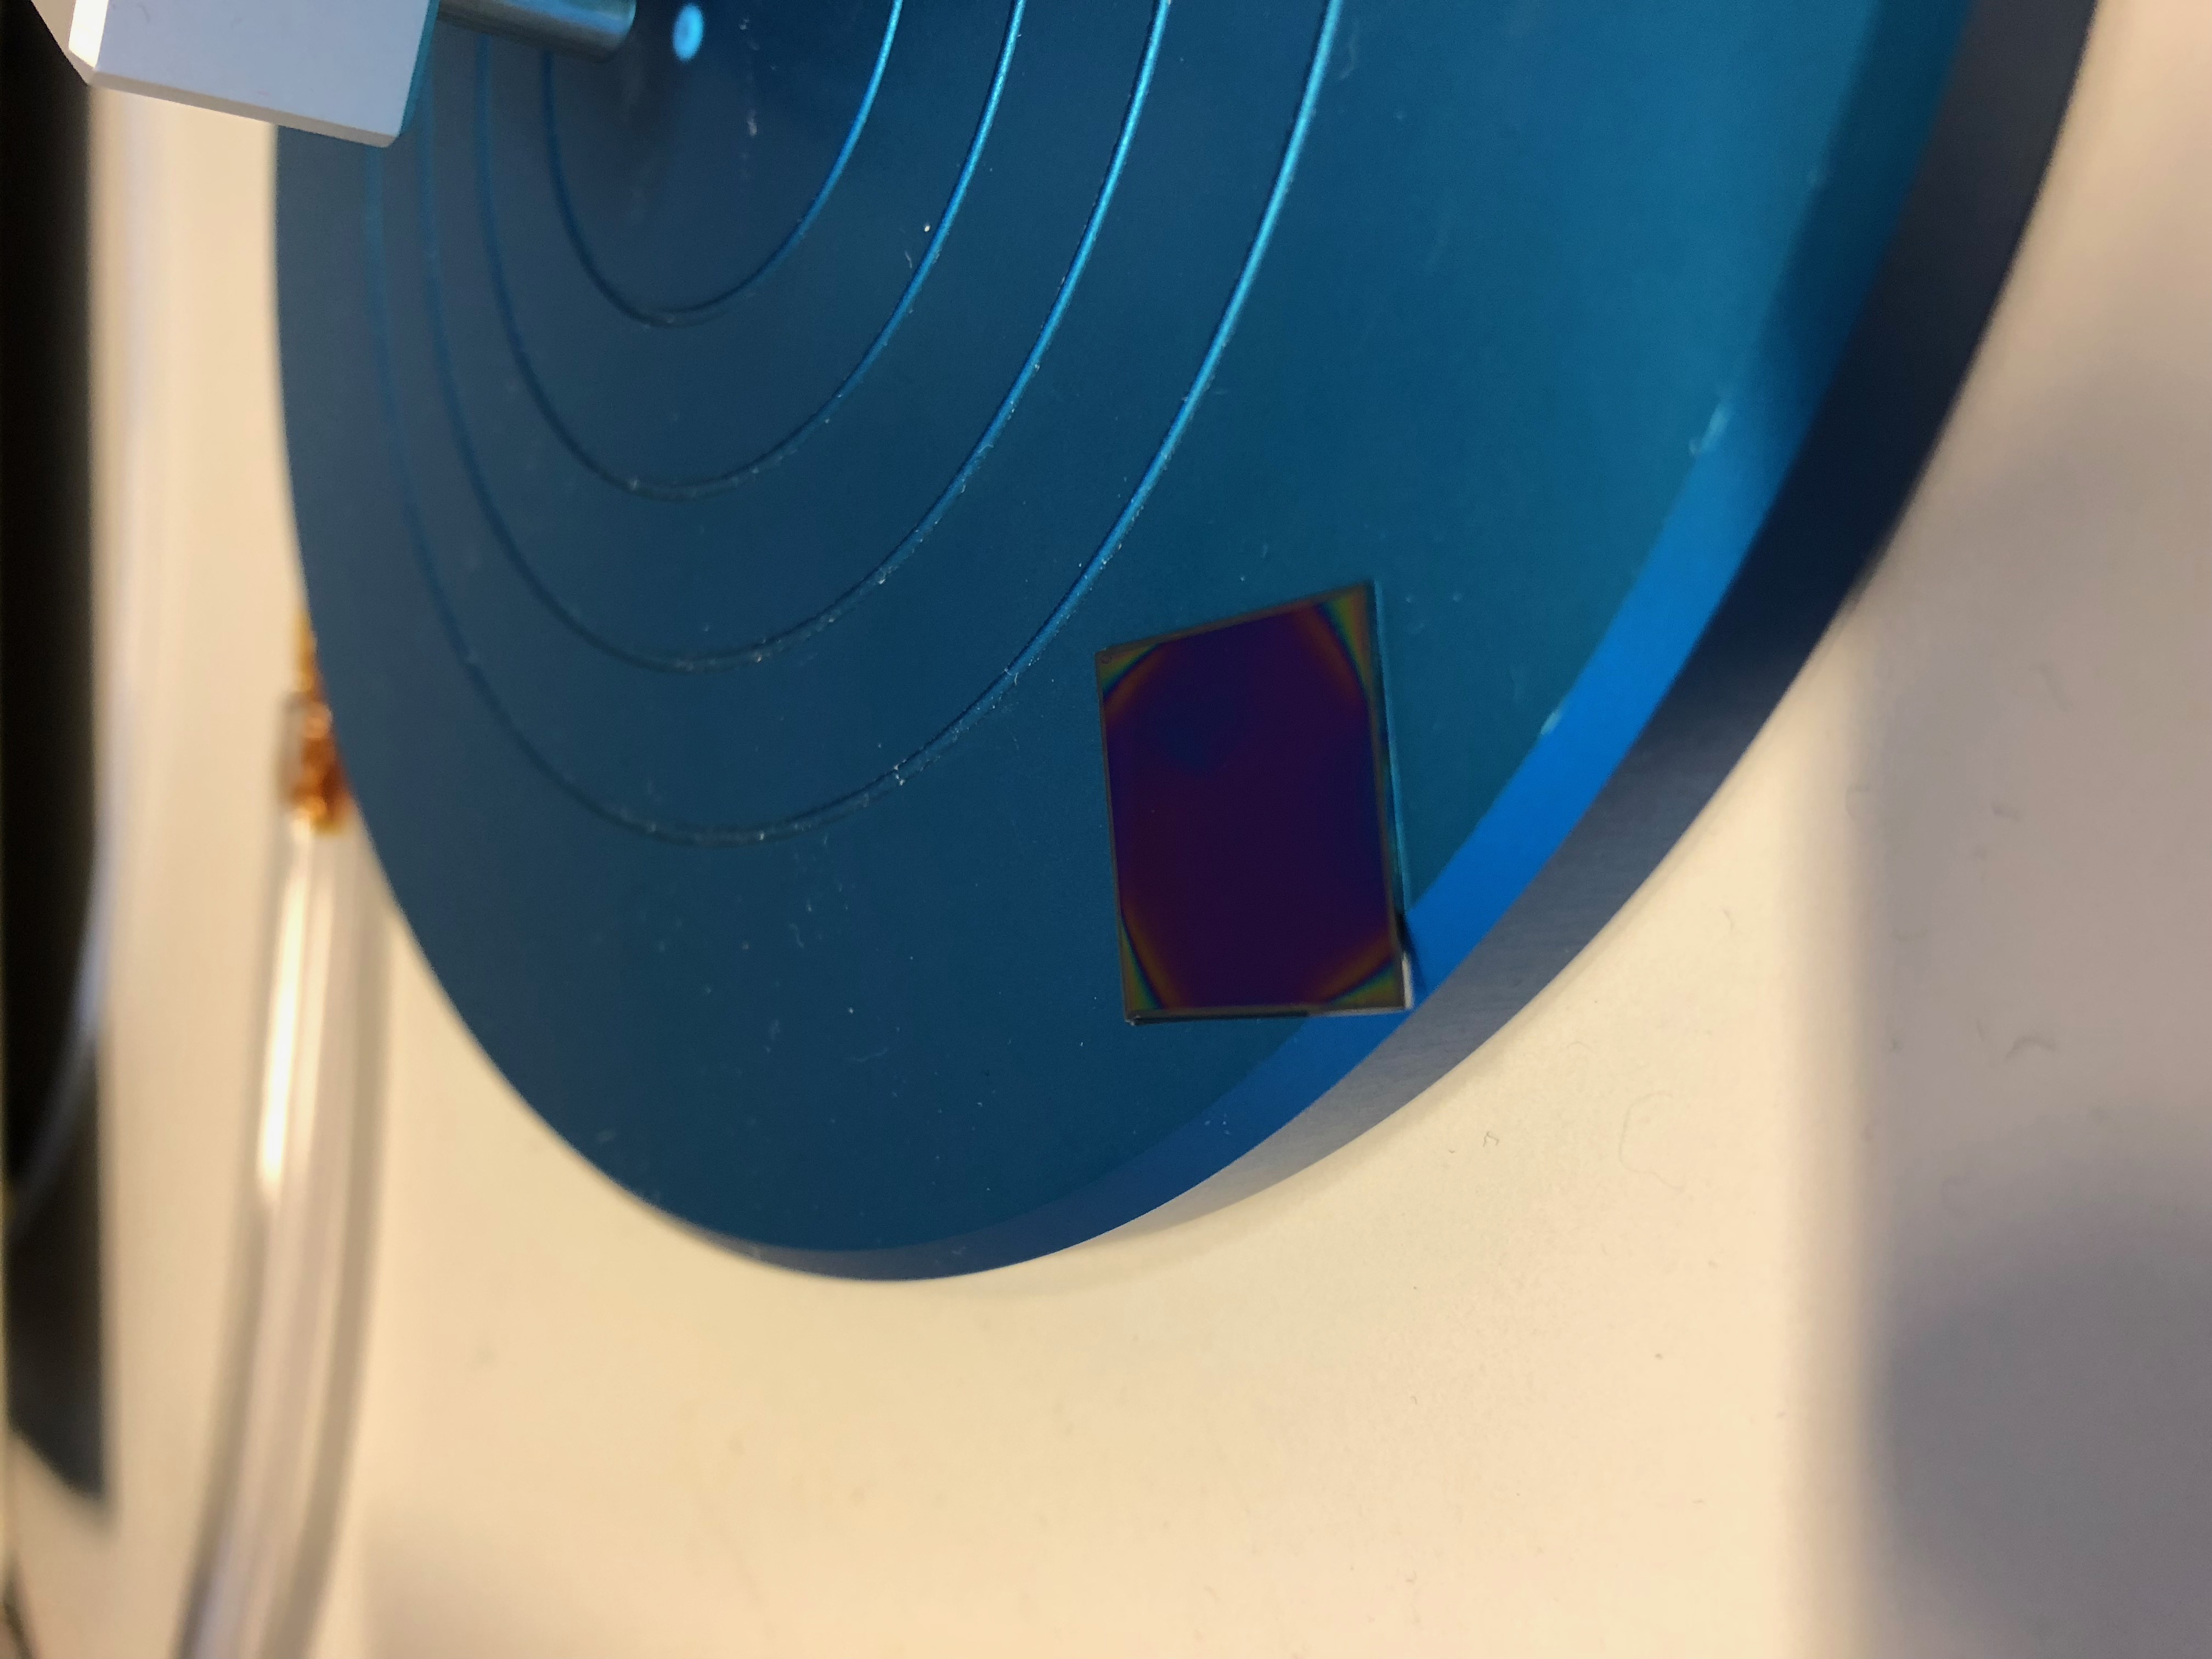
\includegraphics[scale=0.05,angle=-90]{PSthinfilm.JPG}
				\end{figure}
				\end{minipage}	
	\end{frame}
	
	
	%\begin{frame}{NanoCalc Software}
	
	%\begin{figure}
	%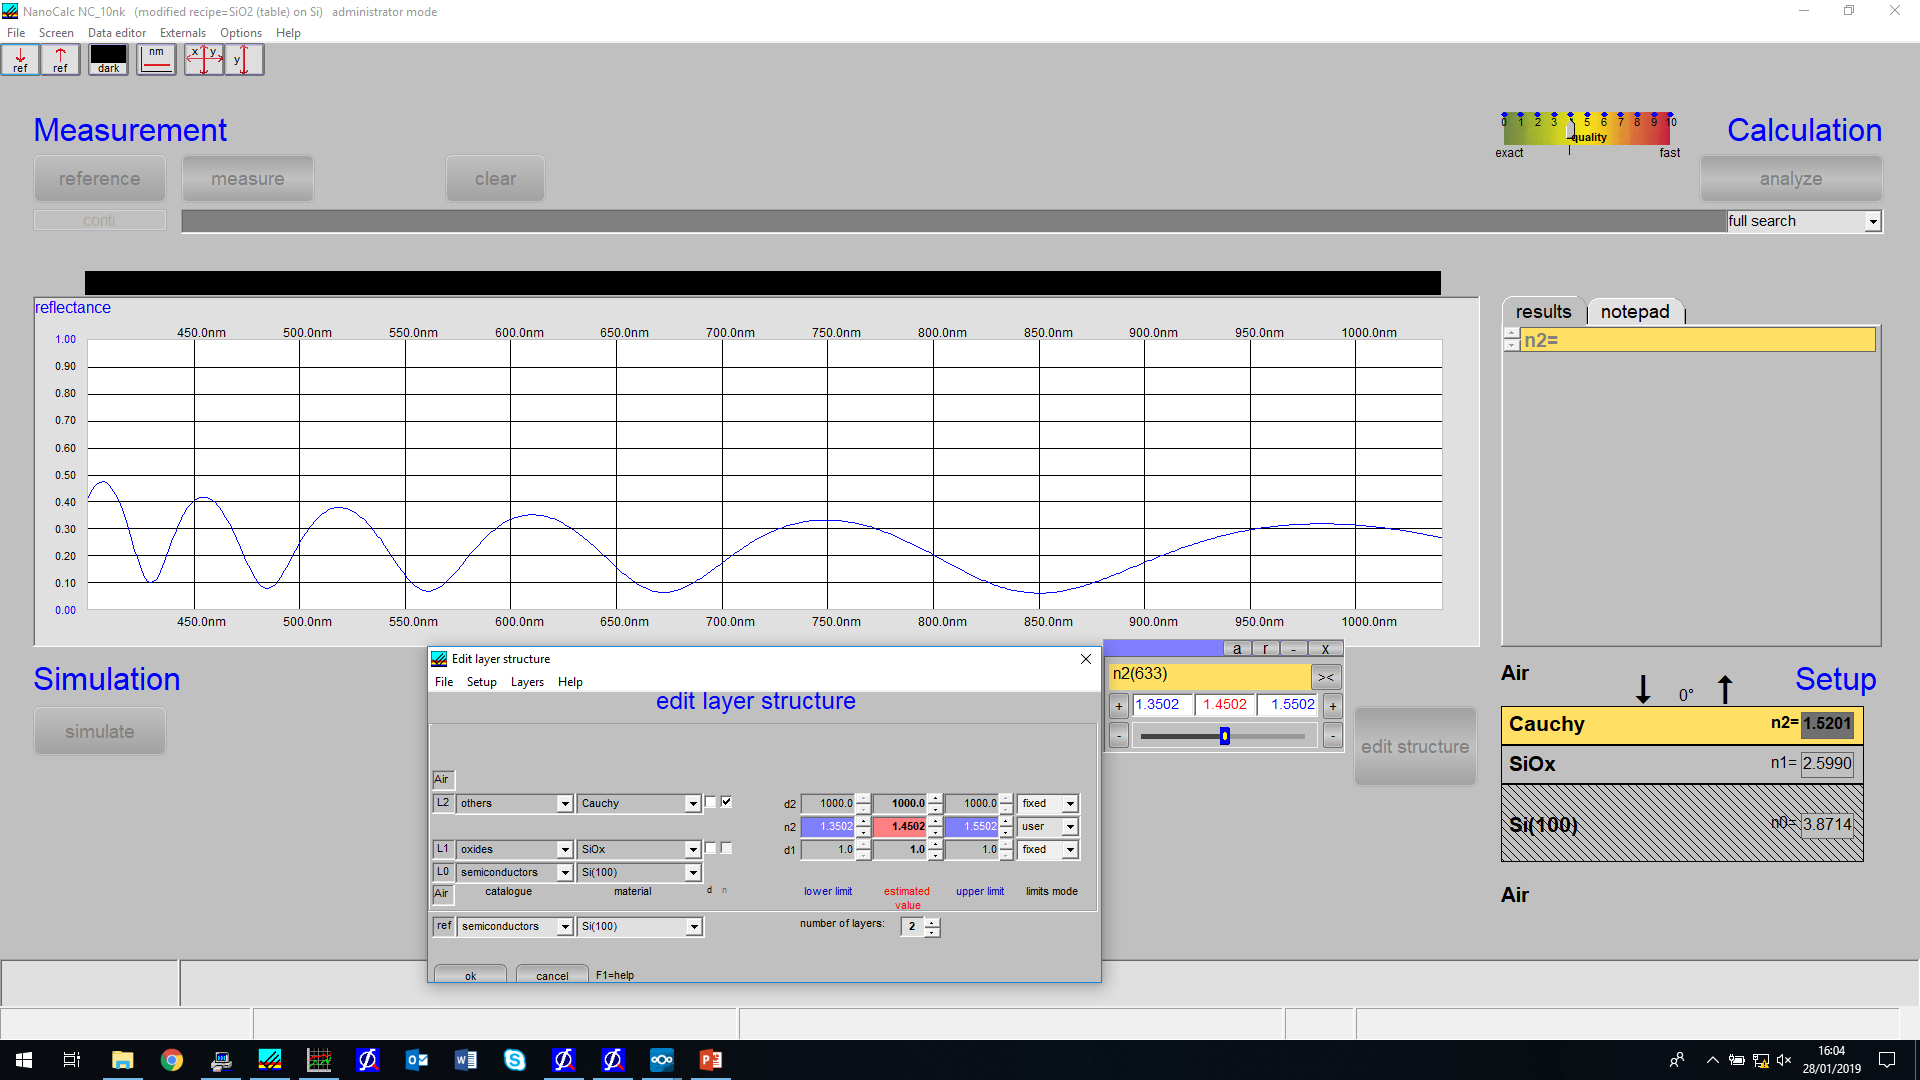
\includegraphics[width=\textwidth]{nanocalc.png}
	%\end{figure}
	
	%\begin{equation*}
	%Reflectance = \frac{Meas-Dark}{Ref} \cdot R_{sub}
	%\end{equation*}
	
	%\end{frame}
	
	\section{Preliminary Models}
	
	\begin{frame}{Fresnel Equations - Substrate}
	
	\begin{minipage}{0.47\textwidth}
	\begin{equation*}
	r_p = \frac{E_{r,p}}{E_{i,p}} = \frac{n_t\cos(\theta_i)-n_i\cos(\theta_t)}{n_i\cos(\theta_t)+n_t\cos(\theta_i)}
	\end{equation*}
	\begin{equation*}
	R_p = \mid r_p \mid ^2 
	\end{equation*}
	\end{minipage}
	\begin{minipage}{0.5\textwidth}
	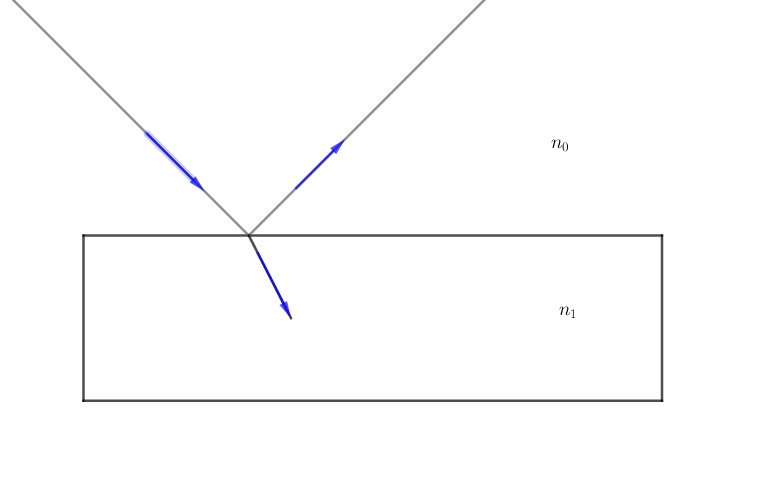
\includegraphics[scale=0.2]{subrefl.png}
	\end{minipage}
	\end{frame}
	
	\begin{frame}{Fresnel Equations - One layer}
	
	\begin{figure} 
		 \begin{center}
		   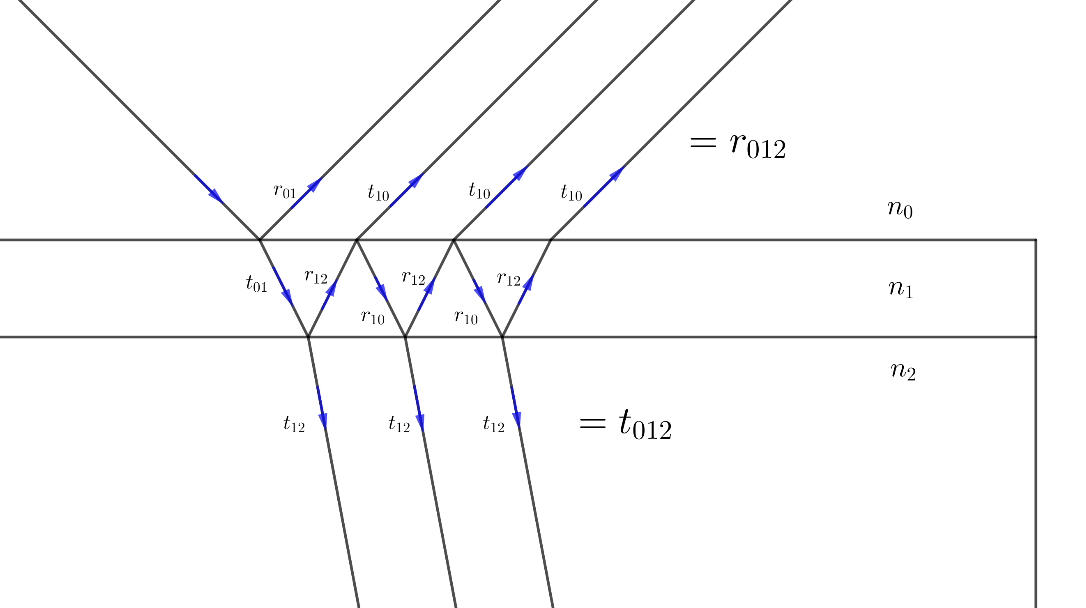
\includegraphics[width=\textwidth]{figreflre.png}
		 \end{center}
	\end{figure}
	\begin{align*}
	r_{012} = &r_{01} + t_{01}t_{10}r_{12}\exp(-i2\beta) + t_{01}t_{10}r_{10}r_{12}^2\exp(-i4\beta)+ \\ &t_{01}t_{10}r_{10}^2r_{12}^3\exp(-i6\beta)+ \cdots
	\end{align*} 
	
	\end{frame}
	
	\begin{frame}{Fresnel Equations - One layer}
	
	\begin{minipage}{0.47\textwidth}
	
	%\begin{equation*} \label{eq:r012big}
	%r_{012}=r_{01}+\frac{t_{01}t_{10}r_{12}\exp(-i2\beta)}{1-r_{10}r_{12}\exp(-i2\beta)}
	%\end{equation*}
		
	\begin{equation*}\label{eq:2layerreflect}
	r_{012}= \frac{r_{01}+r_{12}\exp(-i2\beta)}{1+r_{01}r_{12}\exp(-i2\beta)}
	\end{equation*}
	
	\begin{equation*}
	R_{012} = \mid r_{012} \mid ^2 
	\end{equation*}
	 
	\end{minipage}
	\begin{minipage}{0.5\textwidth}
	\begin{equation*}
	\beta=\frac{2\pi d_1}{\lambda} n_1\cos(\theta_1)
	\end{equation*}
	\end{minipage}	
	\end{frame}
	

\section{Results}

\begin{frame}{Solvent Vapor Annealing of Polystyrene in Toluene}

\end{frame}

\section{Why look at structure?}

\begin{frame}{Structure in thinfilms}
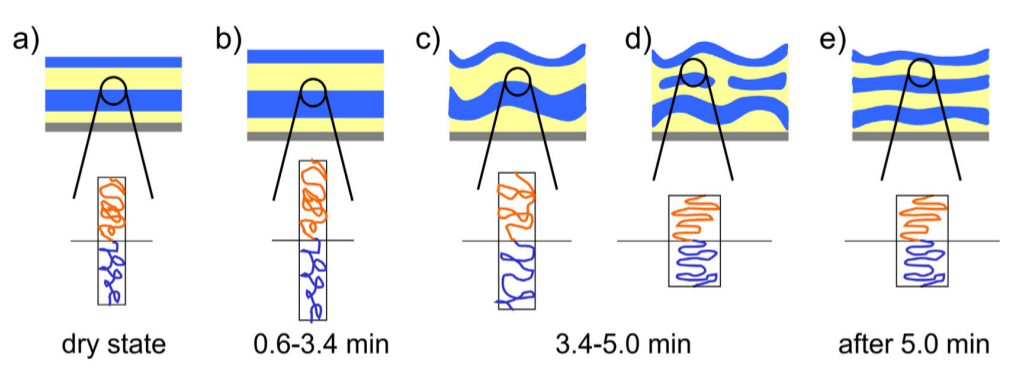
\includegraphics[width=\textwidth]{multipolymer.png}
\end{frame}


\begin{frame}{Structure in Nature}
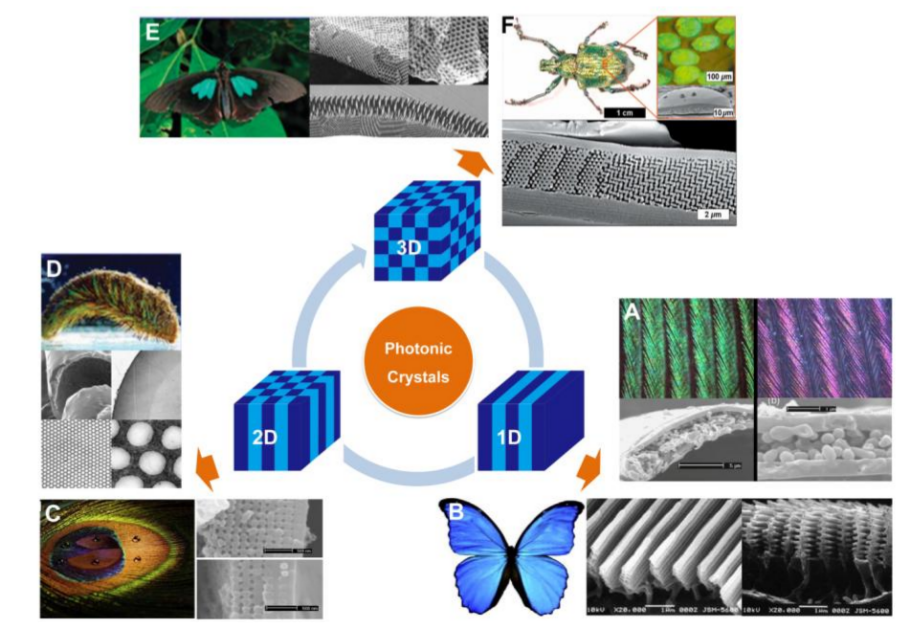
\includegraphics[width=\textwidth]{structure.png}
\end{frame}






%  OLD SLIDES
%
%
%	
%	\begin{frame}{Fresnel equations - multilayers}
%	
%	\begin{figure}
%	\centering
%	\begin{minipage}{0.5\textwidth}
%	\centering
%	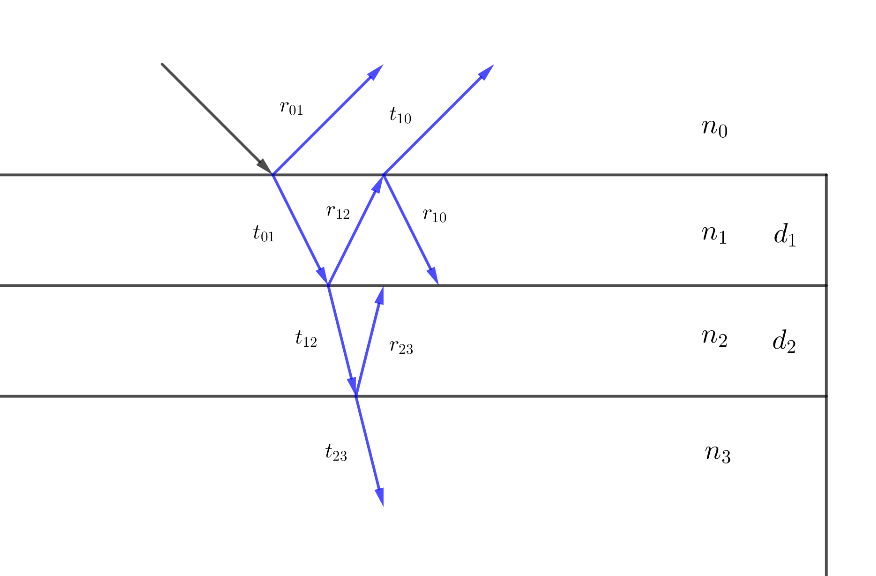
\includegraphics[scale=0.2]{figmulti1re.png}
%	\end{minipage}\quad
%	\begin{minipage}{0.5\textwidth}
%	\begin{figure}
%	\centering
%	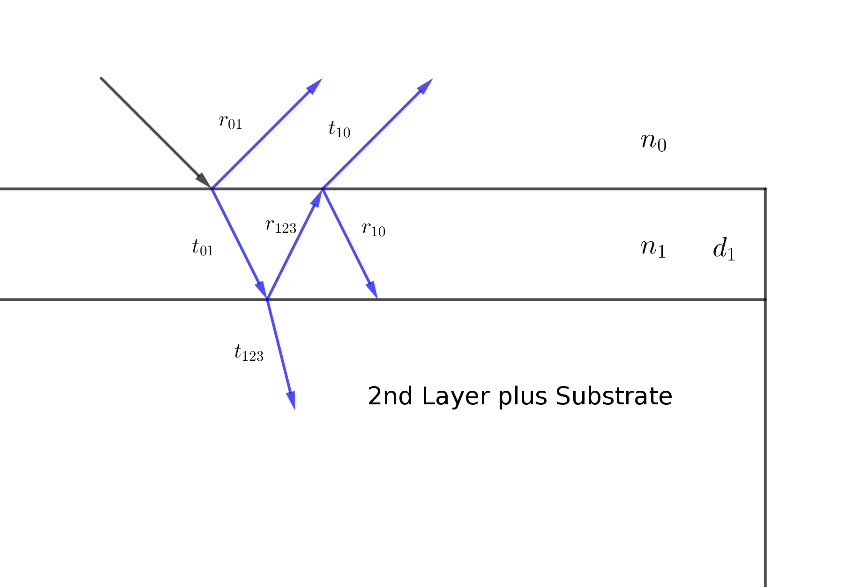
\includegraphics[scale=0.2]{figmulti2re.png}
%	\end{figure}
%	\end{minipage}
%	\end{figure}
%	
%	\end{frame}
%	
%	\begin{frame}{Fresnel equations - multilayers Cont.}
%	
%	\begin{minipage}{0.47\textwidth}
%	\begin{equation*}
%	r_{123}= \frac{r_{12}+r_{23}\exp(-i2\beta_2)}{1+r_{12}r_{23}\exp(-i2\beta_2)}
%	\end{equation*}
%	
%	\begin{equation*}
%	r_{0123}= \frac{r_{01}+r_{123}\exp(-i2\beta_1)}{1+r_{01}r_{123}\exp(-i2\beta_1)}
%	\end{equation*}
%	\end{minipage}
%	\begin{minipage}{0.5\textwidth}
%		\begin{equation*}
%		\beta=\frac{2\pi d}{\lambda} n\cos(\theta)
%		\end{equation*}
%	\end{minipage}
%	\end{frame}
	
%	\begin{frame}{Polymer refractive index dispersion}
%	Cauchy empirical equation for the refractive index in the visible light range.
%	
%	\begin{equation*}
%	n(\lambda) = A + \frac{B}{\lambda^2} + \frac{C}{\lambda^4}
%	\end{equation*}
%	
%	These constants can be found using ellipsometry.
%	
%	Which dispersion to use? Can Cauchy be used for more exotic polymers?   
%	\end{frame}
%	\section{Preliminary Results}
%	
%	\begin{frame}{Substrate Results}
%		\begin{figure}
%		\centering
%		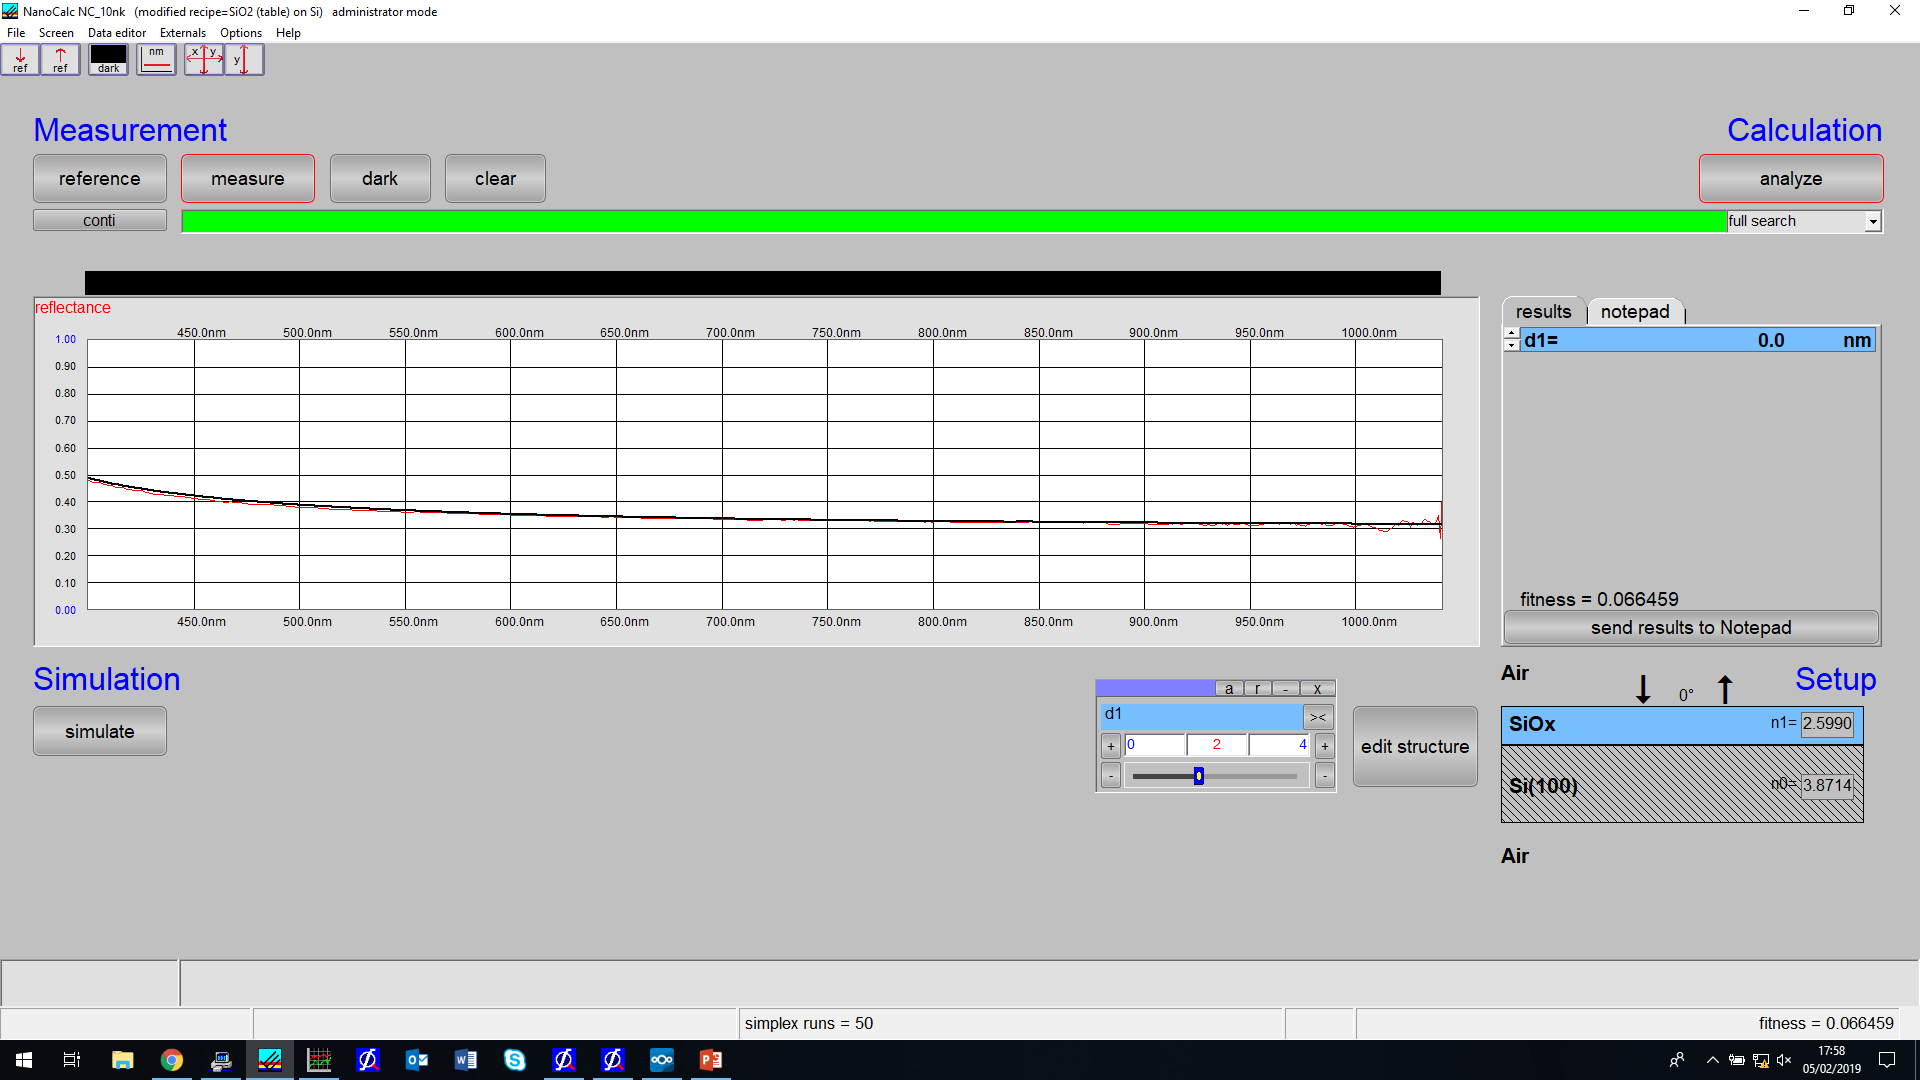
\includegraphics[width=\textwidth]{sub1.png}
%		\end{figure}
%		\end{frame}
%		
%		\begin{frame}{Substrate Results}
%			\begin{figure}
%			\centering
%			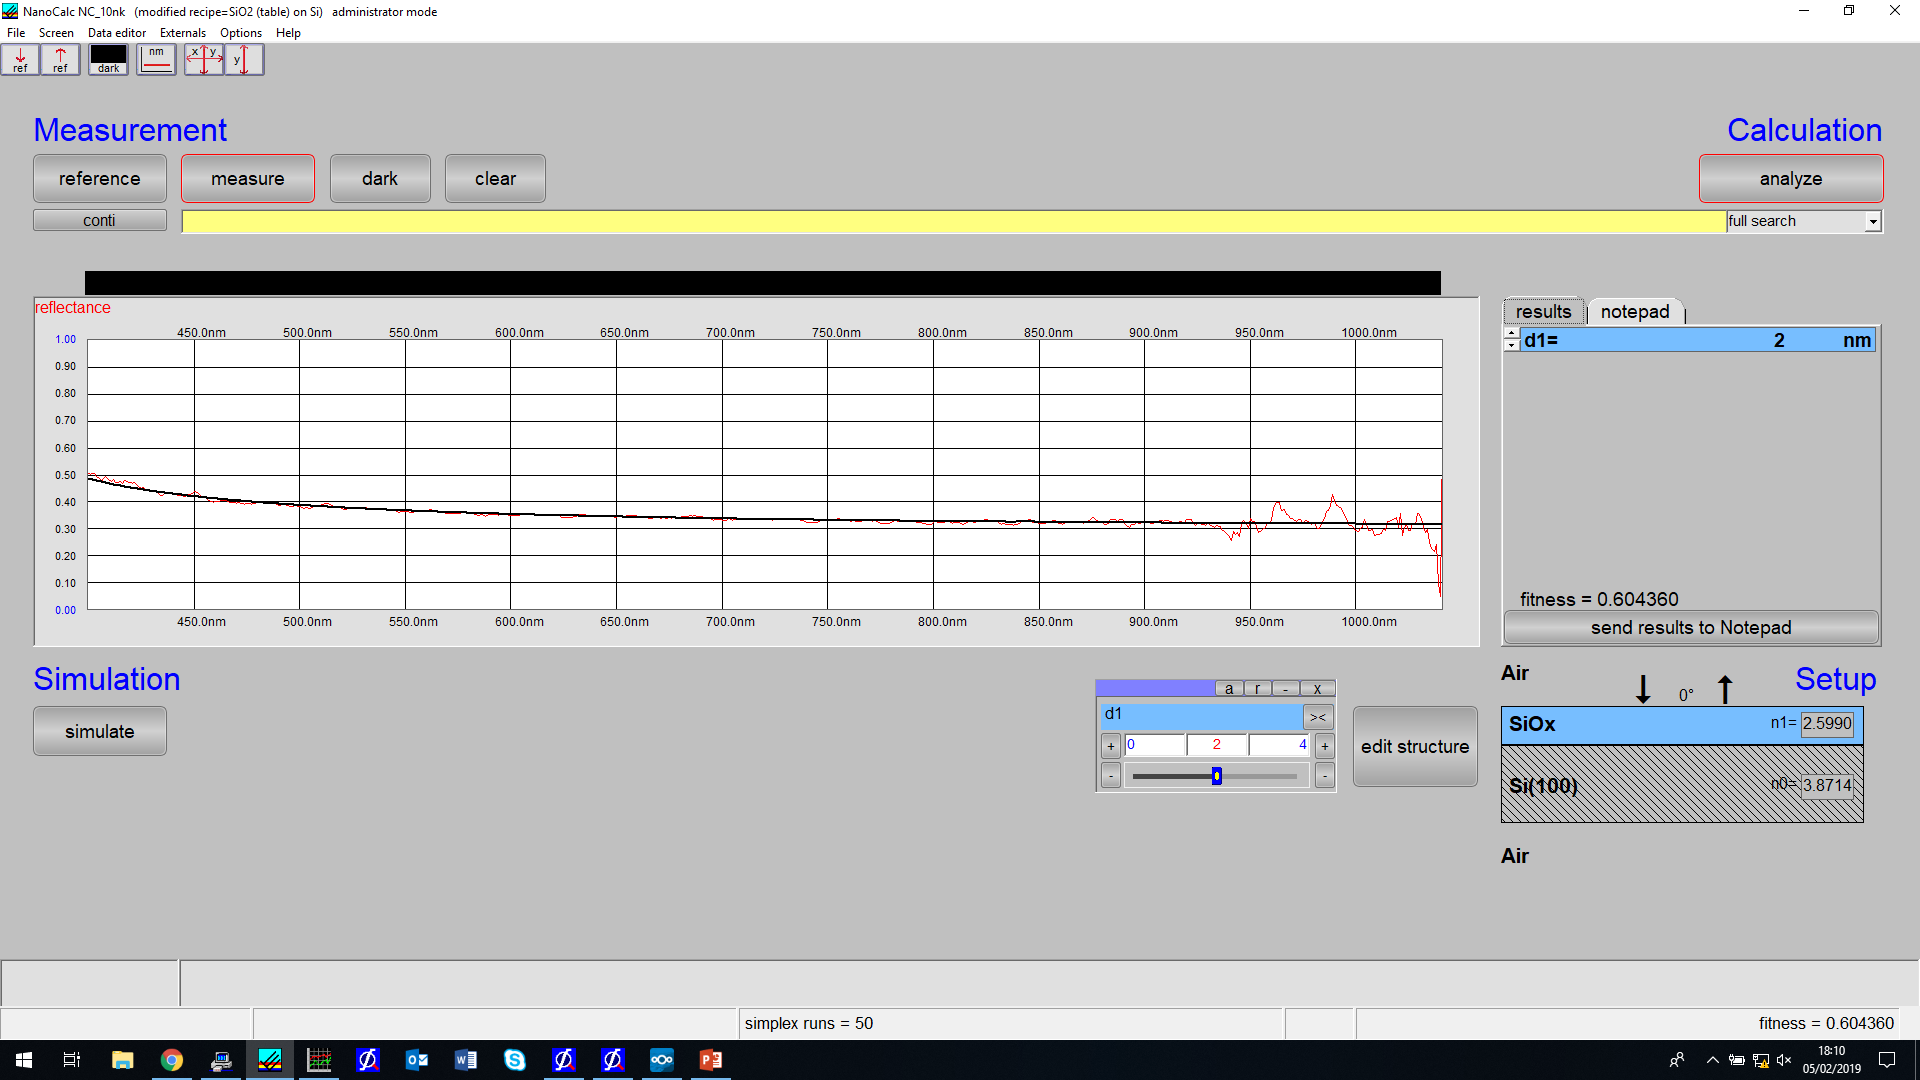
\includegraphics[width=\textwidth]{sub2.png}
%			\end{figure}
%			\end{frame}
%			
%			\begin{frame}{Substrate Results}
%						\begin{figure}
%						\centering
%						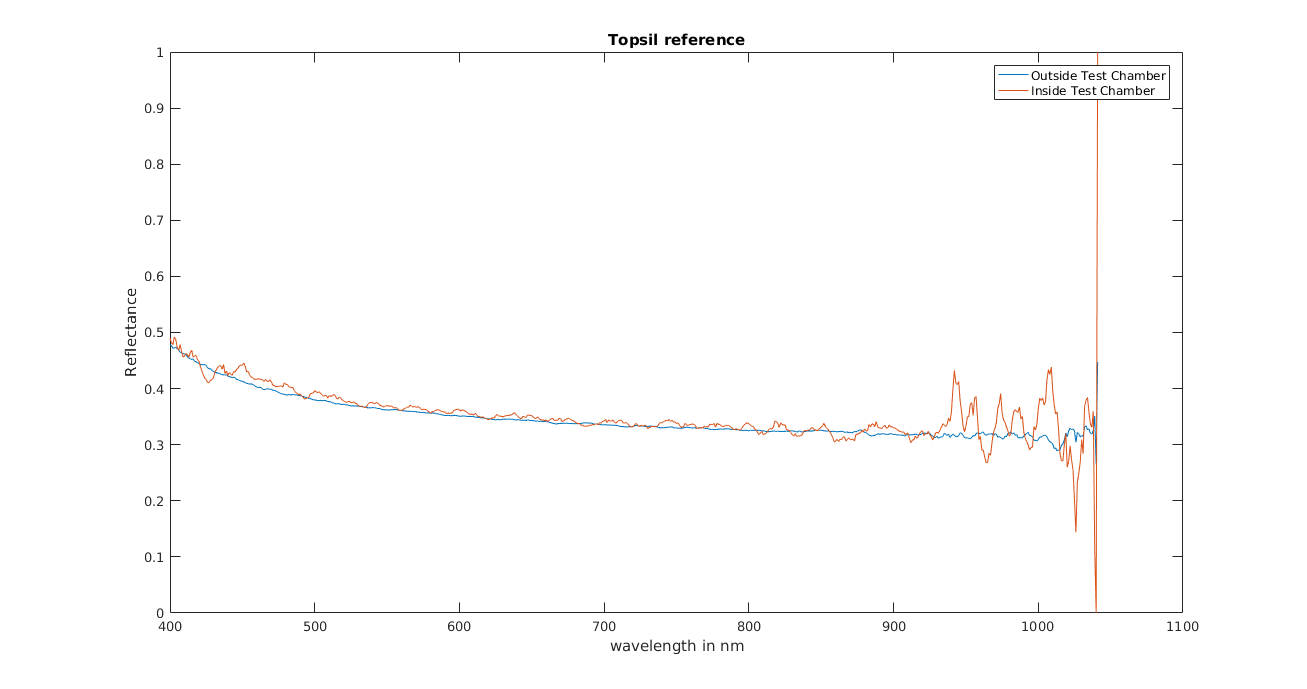
\includegraphics[width=\textwidth]{topsil.png}
%						\end{figure}
%						\end{frame}
%						
%		\begin{frame}{Dark and Ref of Topsil in the test chamber}
%		\begin{figure}
%		\centering
%		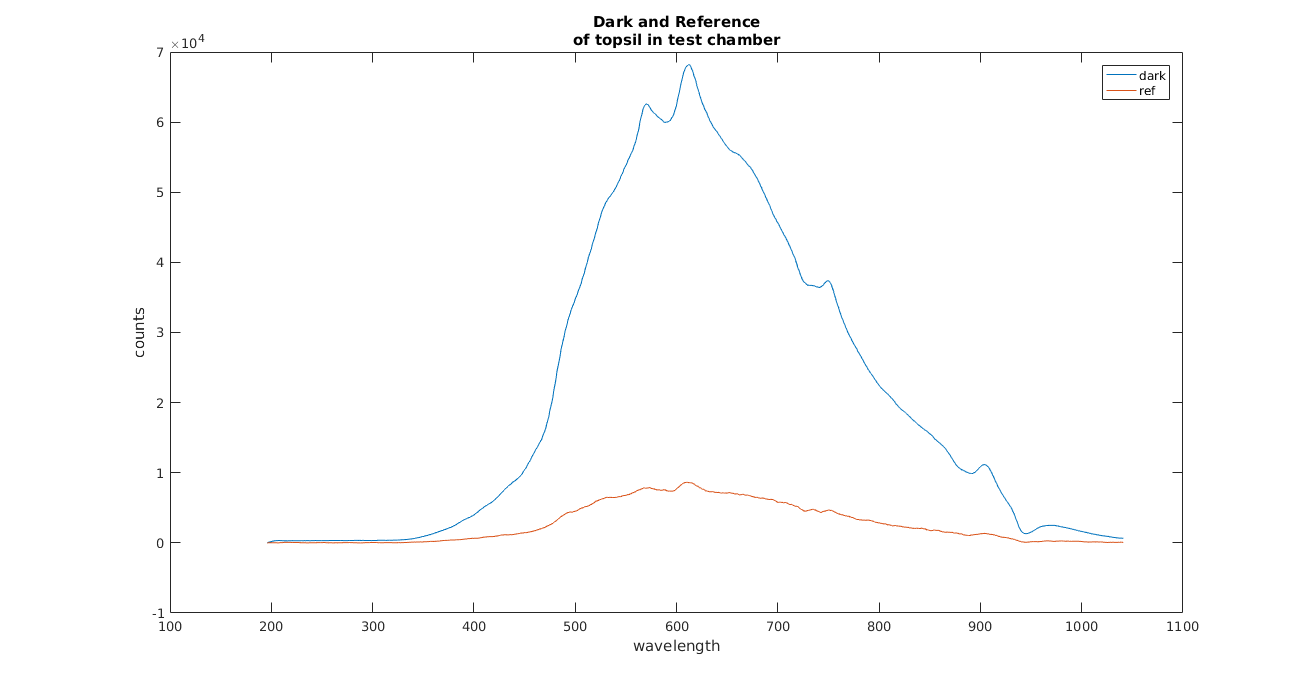
\includegraphics[scale=0.35]{darkref1.png}
%		\end{figure}
%		\end{frame}
%		\begin{frame}{Dark and Ref of Topsil in the test chamber}
%		\begin{figure}
%		\centering
%		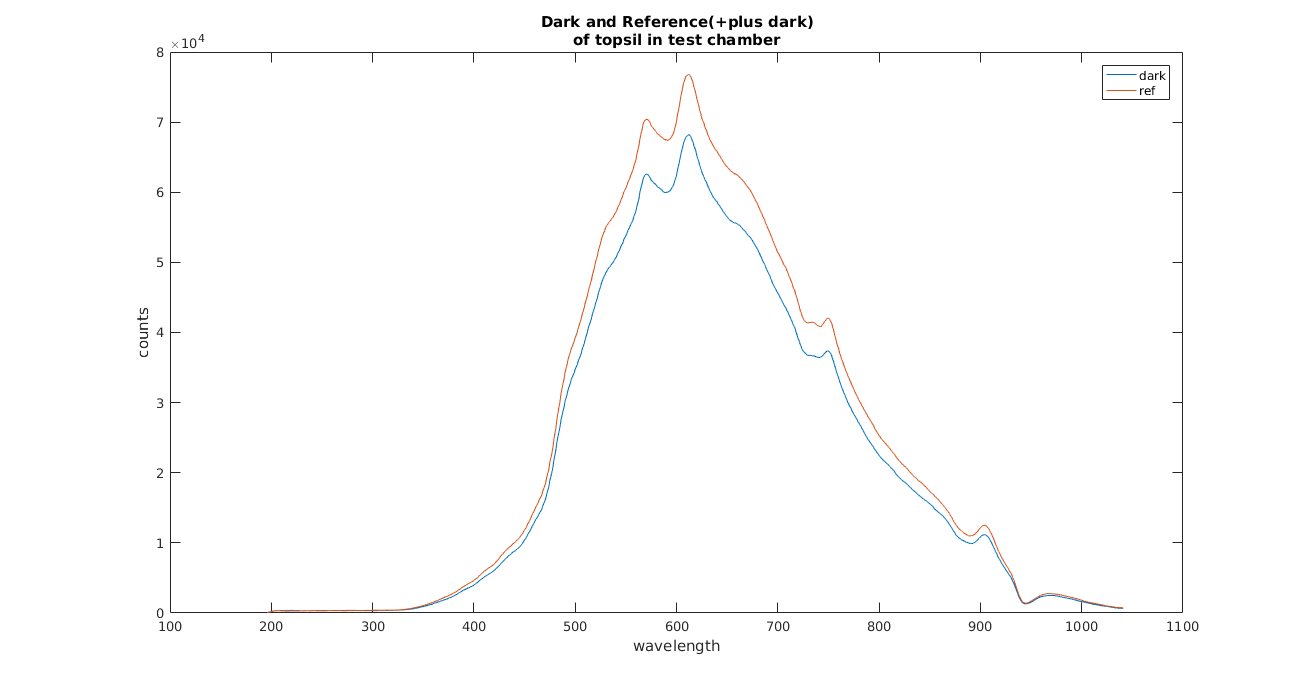
\includegraphics[scale=0.35]{darkref2.png}
%		\end{figure}
%		\end{frame}
%	
%		\begin{frame}{Polystyrene Results}
%			\begin{figure}
%			\centering
%			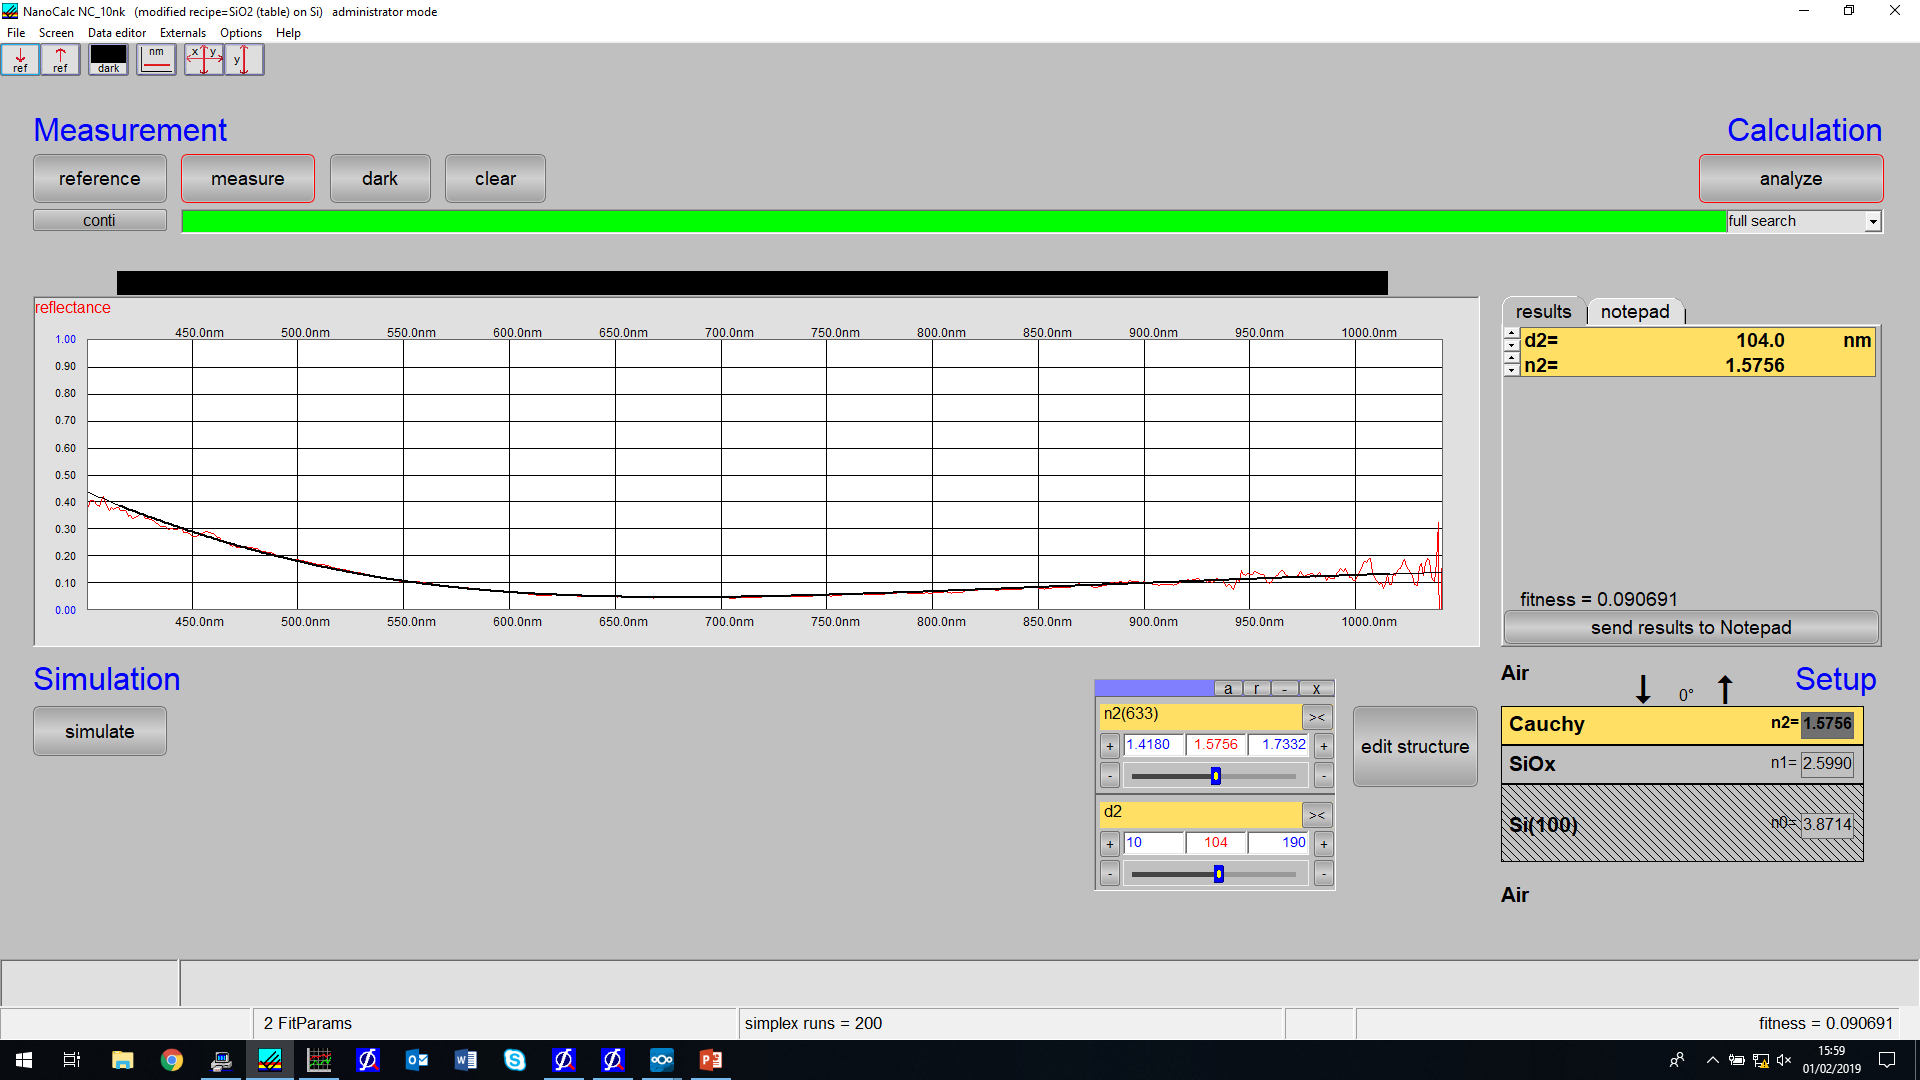
\includegraphics[width=\textwidth]{p1.png}
%			\end{figure}
%			\end{frame}
%	
%	\begin{frame}{Polystyrene Results}
%		\begin{figure}
%		\centering
%		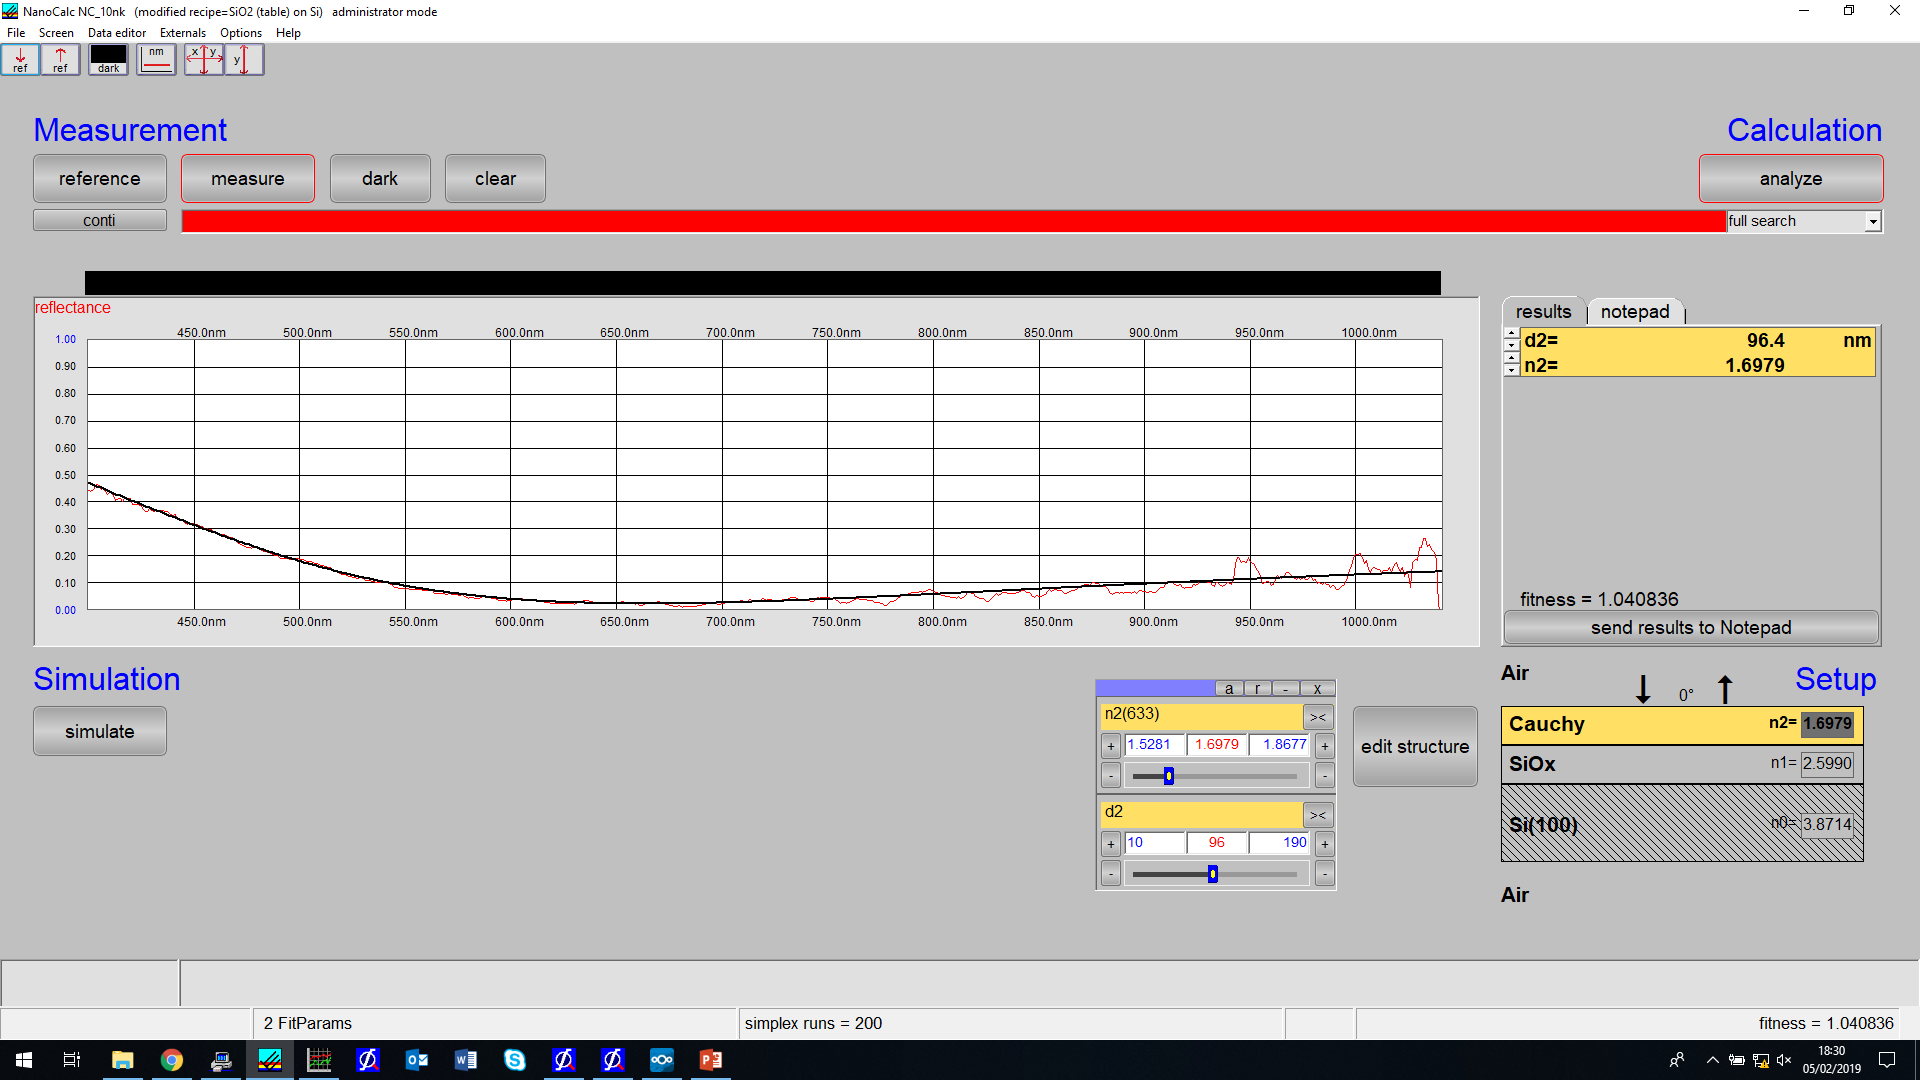
\includegraphics[width=\textwidth]{p2.png}
%		\end{figure}
%	\end{frame}
%	
%	\begin{frame}{Polystyrene Results}
%		\begin{figure}
%		\centering
%		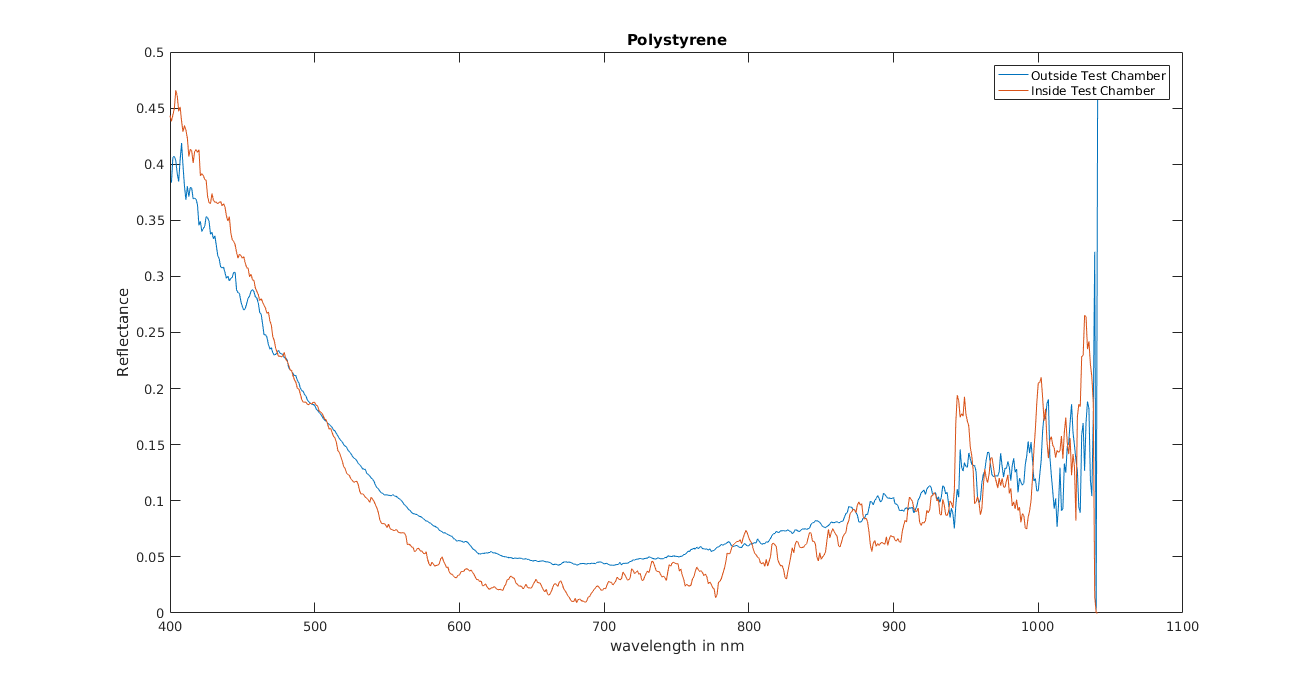
\includegraphics[width=\textwidth]{p3.png}
%		\end{figure}
%		\end{frame}
%		
%		\begin{frame}{Isoprene Results}
%				\begin{figure}
%				\centering
%				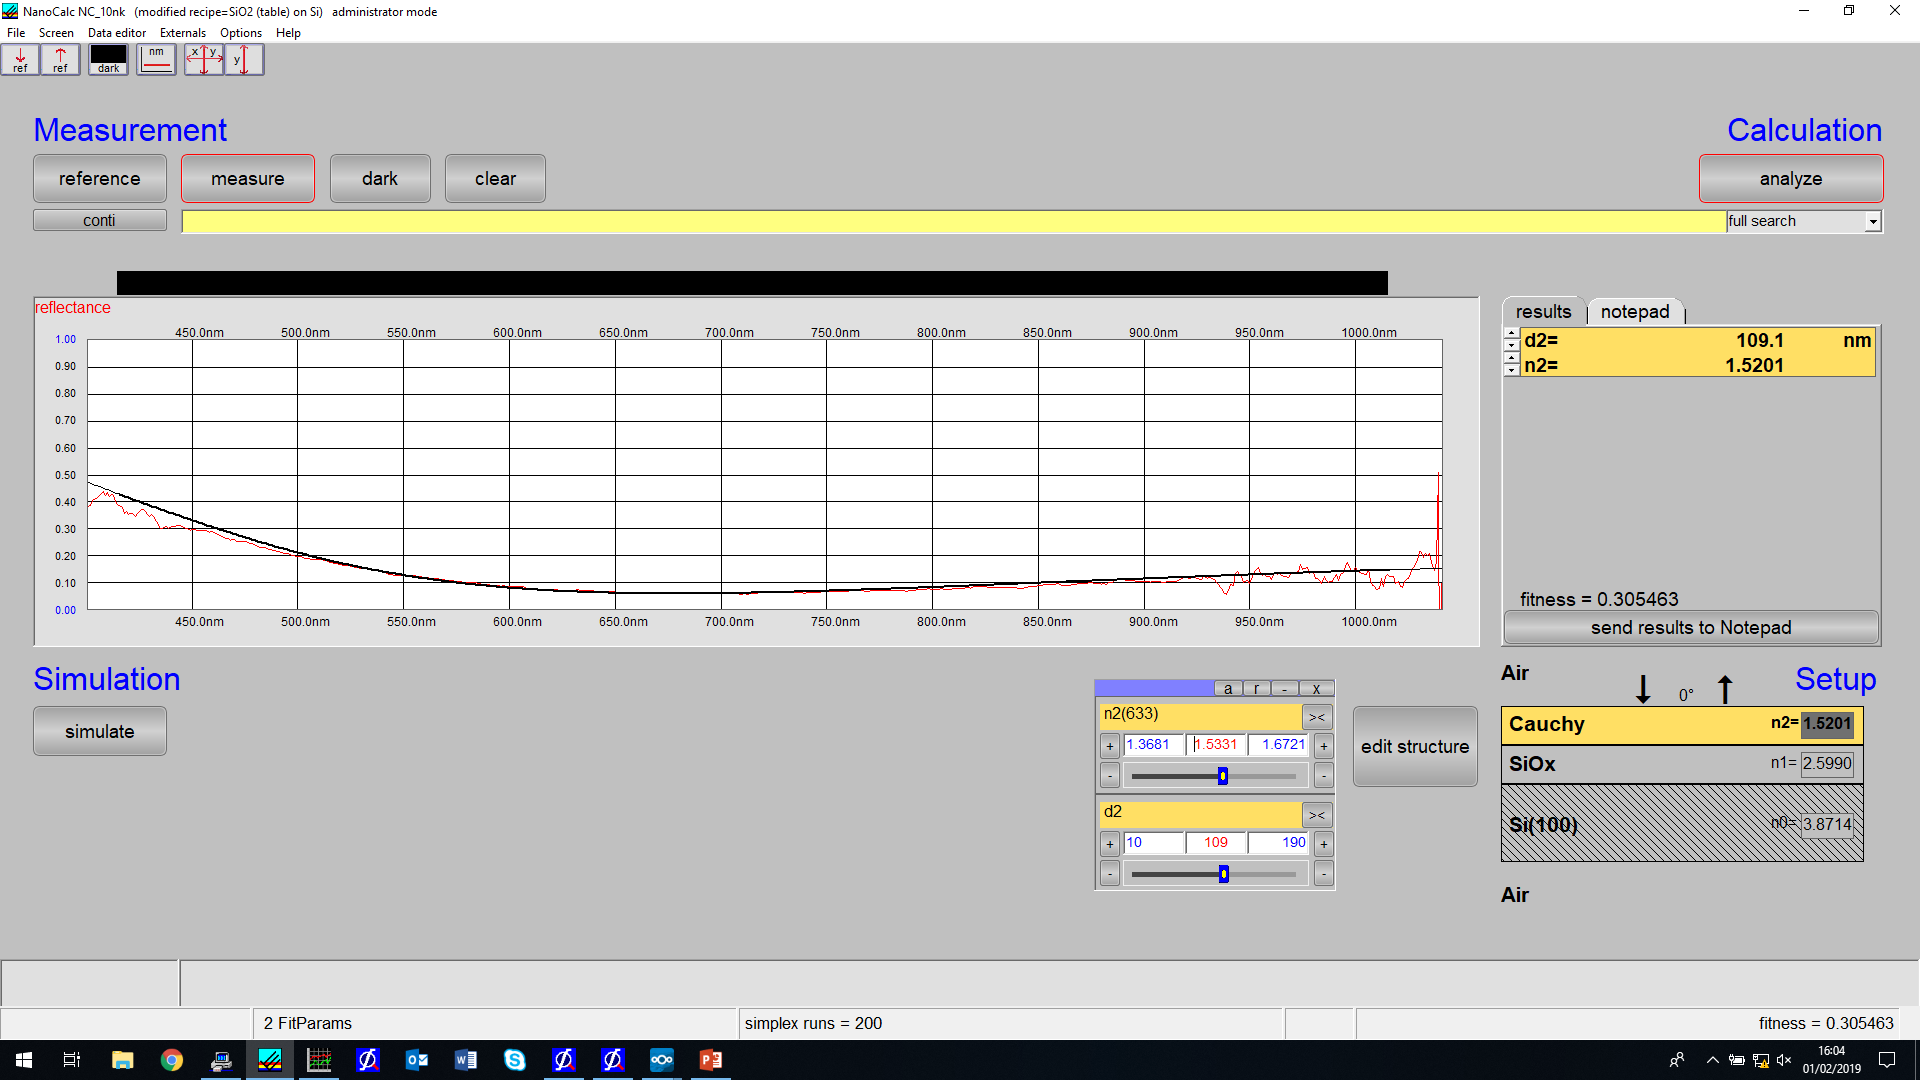
\includegraphics[width=\textwidth]{i1.png}
%				\end{figure}
%				\end{frame}
%				
%\begin{frame}{Isoprene Results}
%\begin{figure}
%\centering
%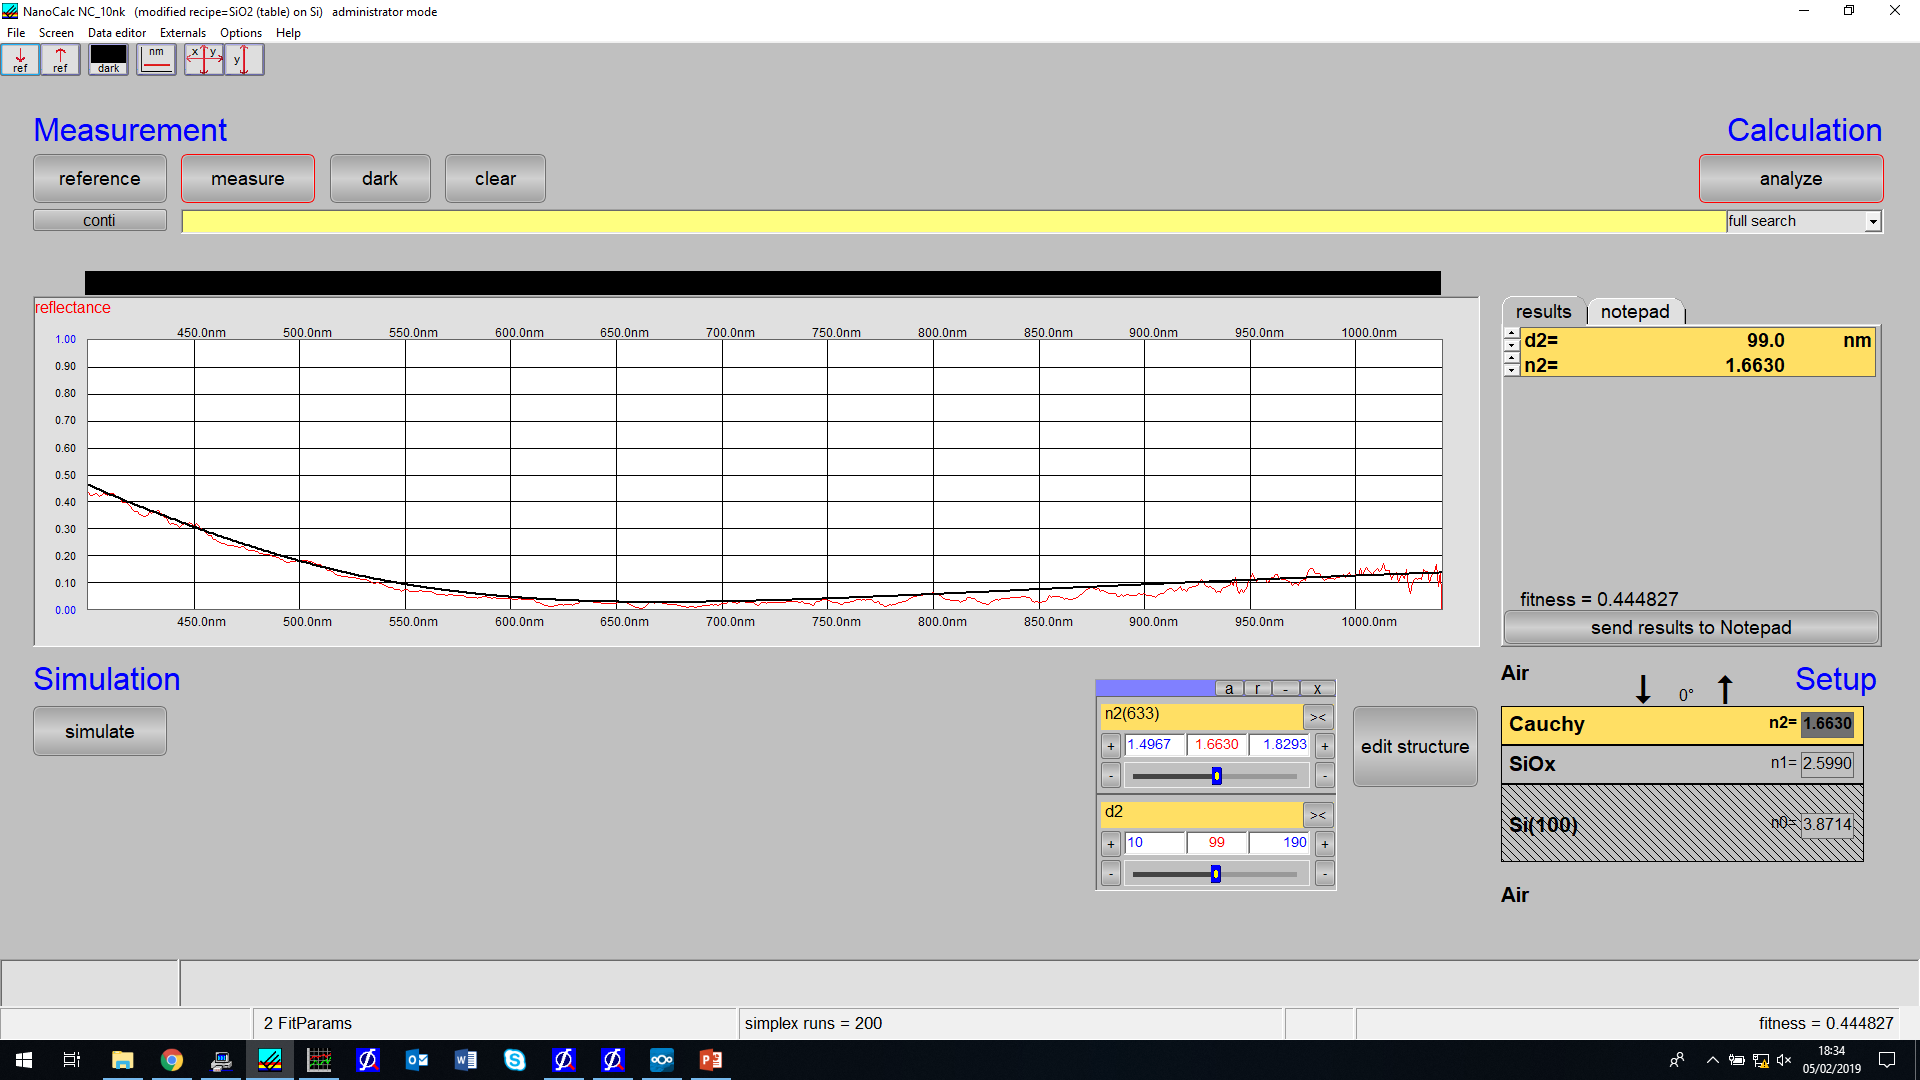
\includegraphics[width=\textwidth]{i2.png}
%\end{figure}
%\end{frame}
%
%\begin{frame}{Isoprene Results}
%\begin{figure}
%\centering
%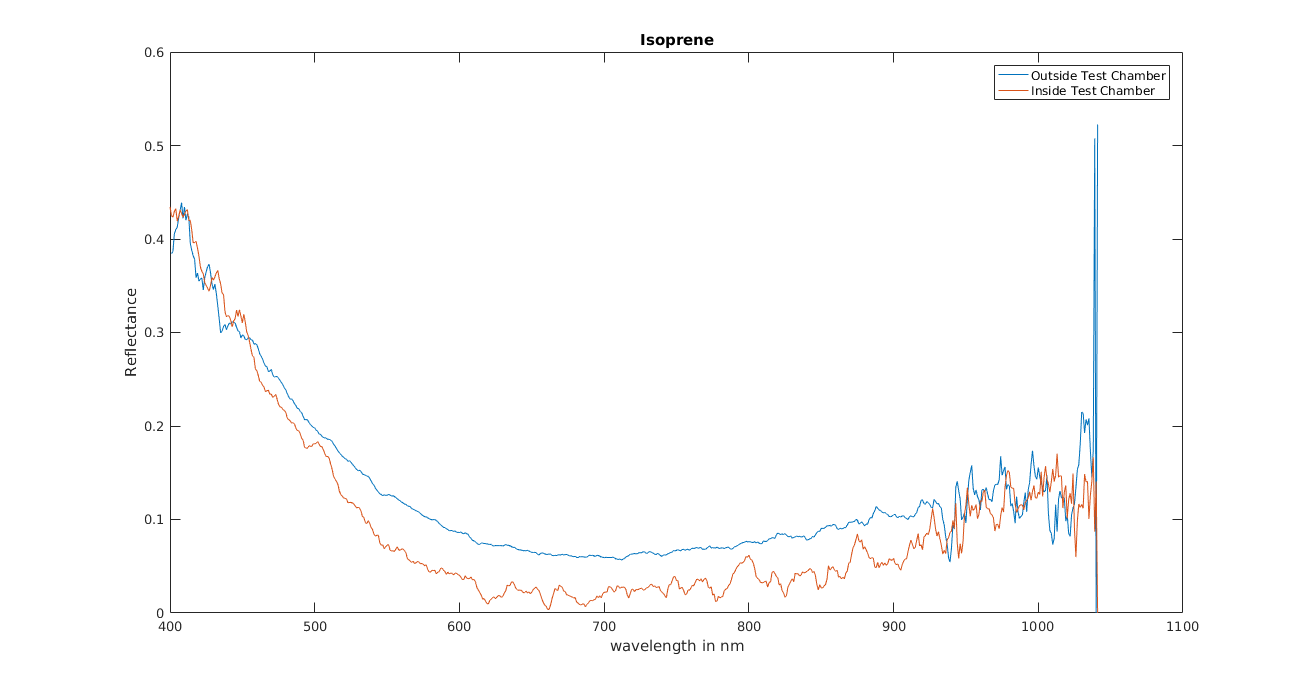
\includegraphics[width=\textwidth]{i3.png}
%\end{figure}
%\end{frame}
%
%\begin{frame}{Methyl Methacrylate Results}
%\begin{figure}
%\centering
%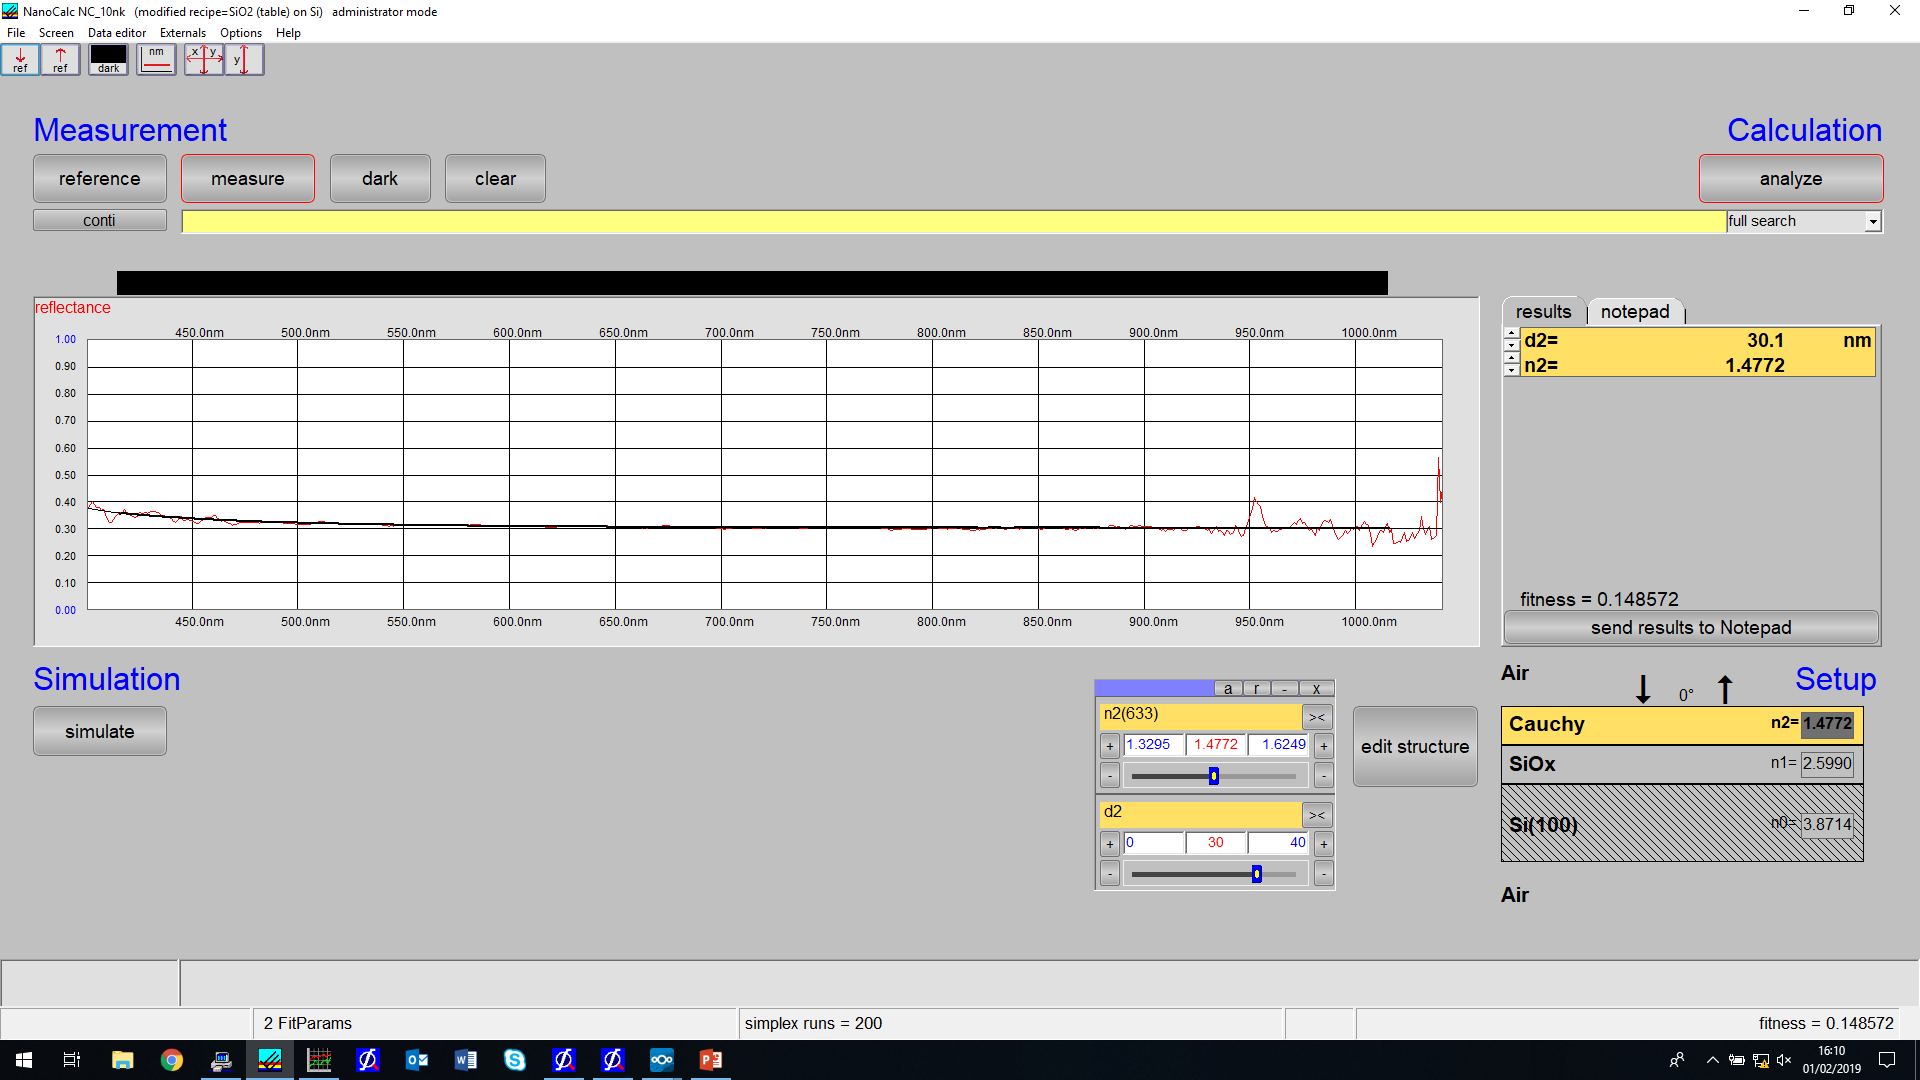
\includegraphics[width=\textwidth]{m1.png}
%\end{figure}
%\end{frame}
%
%\begin{frame}{Methyl Methacrylate Results}
%\begin{figure}
%\centering
%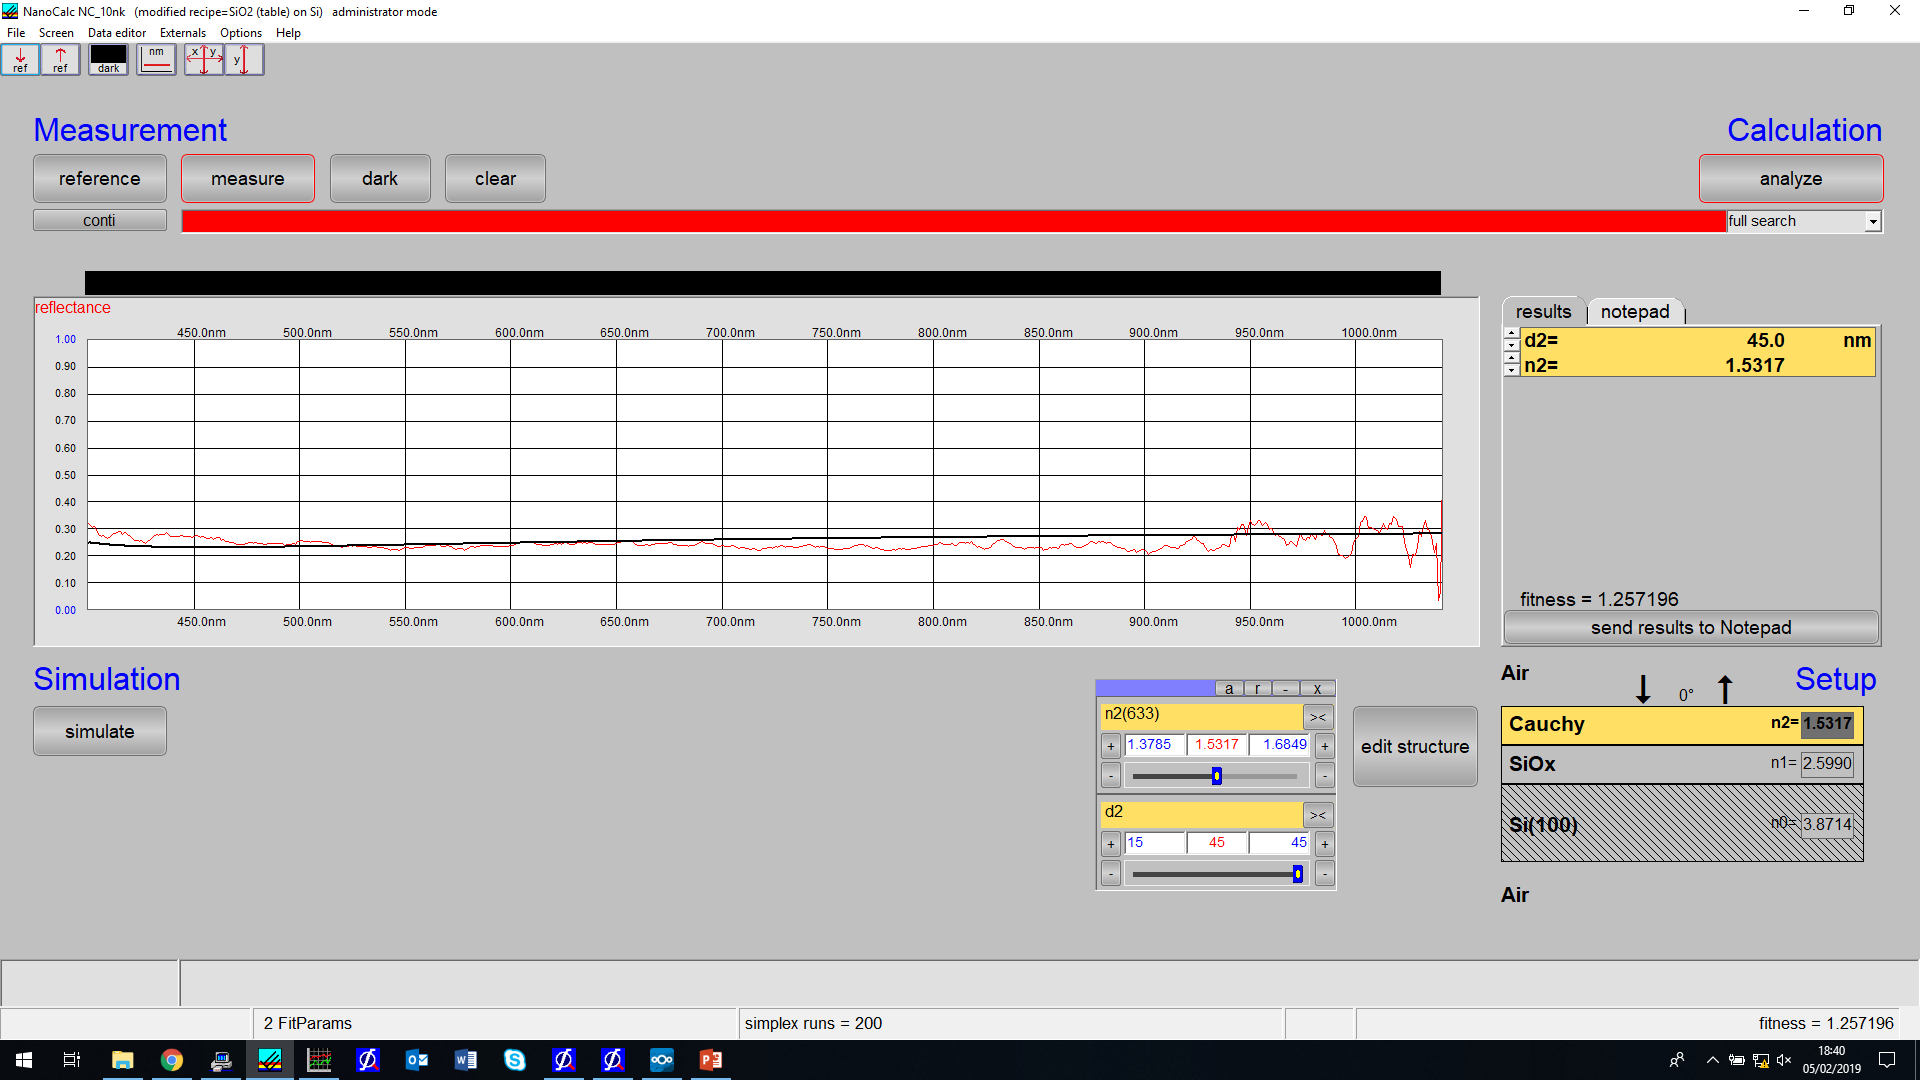
\includegraphics[width=\textwidth]{m2.png}
%\end{figure}
%\end{frame}
%
%\begin{frame}{Methyl Methacrylate Results}
%\begin{figure}
%\centering
%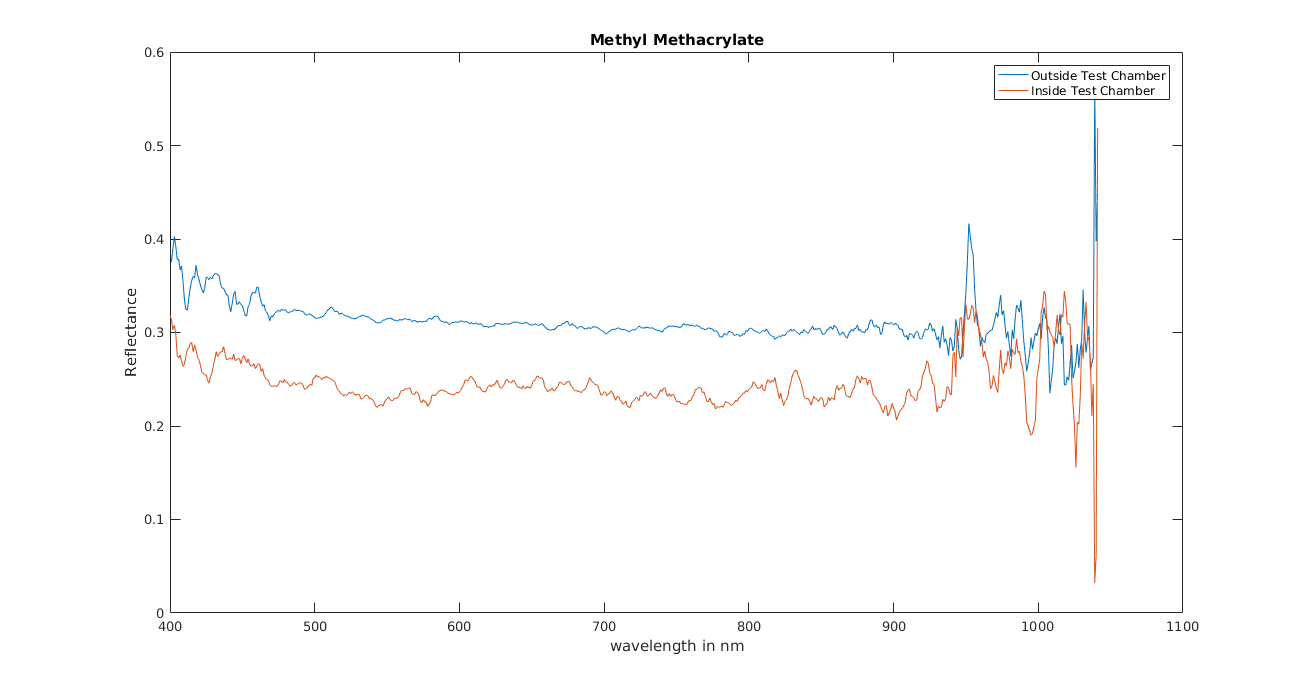
\includegraphics[width=\textwidth]{m3.png}
%\end{figure}
%\end{frame}
%
%\begin{frame}{Future plans}
%\begin{itemize}
%\item Tools to analyse reflectance curves.
%\item Model the lens in test chamber setup.
%\item Refine the experimental protocol.
%\item Investigate the polymers.
%\item Begin to investigate diblock polymers.
%\item Begin to investigate other options for modelling the polymers.
%\end{itemize}
%
%\begin{figure}
%\centering
%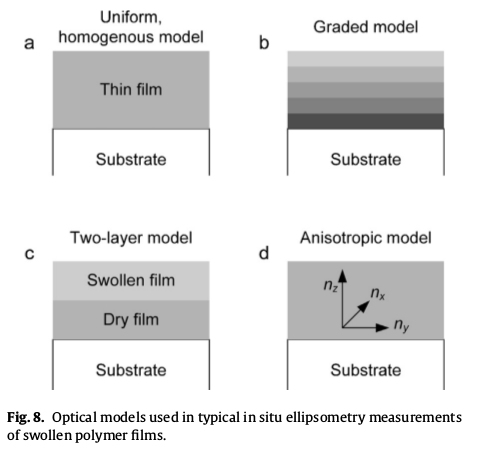
\includegraphics[scale = 0.2]{differentmodels.png}
%\end{figure}
%\end{frame}





\end{document}